% Options for packages loaded elsewhere
\PassOptionsToPackage{unicode}{hyperref}
\PassOptionsToPackage{hyphens}{url}
%
\documentclass[
]{article}
\usepackage{lmodern}
\usepackage{amssymb,amsmath}
\usepackage{ifxetex,ifluatex}
\ifnum 0\ifxetex 1\fi\ifluatex 1\fi=0 % if pdftex
  \usepackage[T1]{fontenc}
  \usepackage[utf8]{inputenc}
  \usepackage{textcomp} % provide euro and other symbols
\else % if luatex or xetex
  \usepackage{unicode-math}
  \defaultfontfeatures{Scale=MatchLowercase}
  \defaultfontfeatures[\rmfamily]{Ligatures=TeX,Scale=1}
\fi
% Use upquote if available, for straight quotes in verbatim environments
\IfFileExists{upquote.sty}{\usepackage{upquote}}{}
\IfFileExists{microtype.sty}{% use microtype if available
  \usepackage[]{microtype}
  \UseMicrotypeSet[protrusion]{basicmath} % disable protrusion for tt fonts
}{}
\makeatletter
\@ifundefined{KOMAClassName}{% if non-KOMA class
  \IfFileExists{parskip.sty}{%
    \usepackage{parskip}
  }{% else
    \setlength{\parindent}{0pt}
    \setlength{\parskip}{6pt plus 2pt minus 1pt}}
}{% if KOMA class
  \KOMAoptions{parskip=half}}
\makeatother
\usepackage{xcolor}
\IfFileExists{xurl.sty}{\usepackage{xurl}}{} % add URL line breaks if available
\IfFileExists{bookmark.sty}{\usepackage{bookmark}}{\usepackage{hyperref}}
\hypersetup{
  pdftitle={Regresion},
  pdfauthor={Ignacio Vellido},
  hidelinks,
  pdfcreator={LaTeX via pandoc}}
\urlstyle{same} % disable monospaced font for URLs
\usepackage[margin=1in]{geometry}
\usepackage{color}
\usepackage{fancyvrb}
\newcommand{\VerbBar}{|}
\newcommand{\VERB}{\Verb[commandchars=\\\{\}]}
\DefineVerbatimEnvironment{Highlighting}{Verbatim}{commandchars=\\\{\}}
% Add ',fontsize=\small' for more characters per line
\usepackage{framed}
\definecolor{shadecolor}{RGB}{248,248,248}
\newenvironment{Shaded}{\begin{snugshade}}{\end{snugshade}}
\newcommand{\AlertTok}[1]{\textcolor[rgb]{0.94,0.16,0.16}{#1}}
\newcommand{\AnnotationTok}[1]{\textcolor[rgb]{0.56,0.35,0.01}{\textbf{\textit{#1}}}}
\newcommand{\AttributeTok}[1]{\textcolor[rgb]{0.77,0.63,0.00}{#1}}
\newcommand{\BaseNTok}[1]{\textcolor[rgb]{0.00,0.00,0.81}{#1}}
\newcommand{\BuiltInTok}[1]{#1}
\newcommand{\CharTok}[1]{\textcolor[rgb]{0.31,0.60,0.02}{#1}}
\newcommand{\CommentTok}[1]{\textcolor[rgb]{0.56,0.35,0.01}{\textit{#1}}}
\newcommand{\CommentVarTok}[1]{\textcolor[rgb]{0.56,0.35,0.01}{\textbf{\textit{#1}}}}
\newcommand{\ConstantTok}[1]{\textcolor[rgb]{0.00,0.00,0.00}{#1}}
\newcommand{\ControlFlowTok}[1]{\textcolor[rgb]{0.13,0.29,0.53}{\textbf{#1}}}
\newcommand{\DataTypeTok}[1]{\textcolor[rgb]{0.13,0.29,0.53}{#1}}
\newcommand{\DecValTok}[1]{\textcolor[rgb]{0.00,0.00,0.81}{#1}}
\newcommand{\DocumentationTok}[1]{\textcolor[rgb]{0.56,0.35,0.01}{\textbf{\textit{#1}}}}
\newcommand{\ErrorTok}[1]{\textcolor[rgb]{0.64,0.00,0.00}{\textbf{#1}}}
\newcommand{\ExtensionTok}[1]{#1}
\newcommand{\FloatTok}[1]{\textcolor[rgb]{0.00,0.00,0.81}{#1}}
\newcommand{\FunctionTok}[1]{\textcolor[rgb]{0.00,0.00,0.00}{#1}}
\newcommand{\ImportTok}[1]{#1}
\newcommand{\InformationTok}[1]{\textcolor[rgb]{0.56,0.35,0.01}{\textbf{\textit{#1}}}}
\newcommand{\KeywordTok}[1]{\textcolor[rgb]{0.13,0.29,0.53}{\textbf{#1}}}
\newcommand{\NormalTok}[1]{#1}
\newcommand{\OperatorTok}[1]{\textcolor[rgb]{0.81,0.36,0.00}{\textbf{#1}}}
\newcommand{\OtherTok}[1]{\textcolor[rgb]{0.56,0.35,0.01}{#1}}
\newcommand{\PreprocessorTok}[1]{\textcolor[rgb]{0.56,0.35,0.01}{\textit{#1}}}
\newcommand{\RegionMarkerTok}[1]{#1}
\newcommand{\SpecialCharTok}[1]{\textcolor[rgb]{0.00,0.00,0.00}{#1}}
\newcommand{\SpecialStringTok}[1]{\textcolor[rgb]{0.31,0.60,0.02}{#1}}
\newcommand{\StringTok}[1]{\textcolor[rgb]{0.31,0.60,0.02}{#1}}
\newcommand{\VariableTok}[1]{\textcolor[rgb]{0.00,0.00,0.00}{#1}}
\newcommand{\VerbatimStringTok}[1]{\textcolor[rgb]{0.31,0.60,0.02}{#1}}
\newcommand{\WarningTok}[1]{\textcolor[rgb]{0.56,0.35,0.01}{\textbf{\textit{#1}}}}
\usepackage{longtable,booktabs}
% Correct order of tables after \paragraph or \subparagraph
\usepackage{etoolbox}
\makeatletter
\patchcmd\longtable{\par}{\if@noskipsec\mbox{}\fi\par}{}{}
\makeatother
% Allow footnotes in longtable head/foot
\IfFileExists{footnotehyper.sty}{\usepackage{footnotehyper}}{\usepackage{footnote}}
\makesavenoteenv{longtable}
\usepackage{graphicx,grffile}
\makeatletter
\def\maxwidth{\ifdim\Gin@nat@width>\linewidth\linewidth\else\Gin@nat@width\fi}
\def\maxheight{\ifdim\Gin@nat@height>\textheight\textheight\else\Gin@nat@height\fi}
\makeatother
% Scale images if necessary, so that they will not overflow the page
% margins by default, and it is still possible to overwrite the defaults
% using explicit options in \includegraphics[width, height, ...]{}
\setkeys{Gin}{width=\maxwidth,height=\maxheight,keepaspectratio}
% Set default figure placement to htbp
\makeatletter
\def\fps@figure{htbp}
\makeatother
\setlength{\emergencystretch}{3em} % prevent overfull lines
\providecommand{\tightlist}{%
  \setlength{\itemsep}{0pt}\setlength{\parskip}{0pt}}
\setcounter{secnumdepth}{-\maxdimen} % remove section numbering

\title{Regresion}
\author{Ignacio Vellido}
\date{11/17/2020}

\begin{document}
\maketitle

Cargamos los datos:

\begin{Shaded}
\begin{Highlighting}[]
\NormalTok{names <-}\StringTok{ }\KeywordTok{c}\NormalTok{(}\StringTok{"Displacement"}\NormalTok{, }\StringTok{"Horse_power"}\NormalTok{, }\StringTok{"Weight"}\NormalTok{, }\StringTok{"Acceleration"}\NormalTok{, }\StringTok{"Model_year"}\NormalTok{, }\StringTok{"Mpg"}\NormalTok{)}

\NormalTok{auto <-}\StringTok{ }\KeywordTok{read_csv}\NormalTok{(}\StringTok{"Data/autoMPG6/autoMPG6.dat"}\NormalTok{, }\DataTypeTok{comment =} \StringTok{"@"}\NormalTok{, }\DataTypeTok{col_names =}\NormalTok{ names)}
\end{Highlighting}
\end{Shaded}

\begin{verbatim}

-- Column specification --------------------------------------------------------
cols(
  Displacement = col_double(),
  Horse_power = col_double(),
  Weight = col_double(),
  Acceleration = col_double(),
  Model_year = col_double(),
  Mpg = col_double()
)
\end{verbatim}

\begin{center}\rule{0.5\linewidth}{0.5pt}\end{center}

Recordamos que la descripción de los datos se encuentra en el apartado
{[}??{]}

Como se comentó en el apartado de EDA:

``Se nos pide elegir 5 regresores para la regresión y contamos
exactamente con ese número, por lo que no podemos descartar ninguna
variable. Aún así, hemos visto que tenemos algunas variables más
interesentas que otras. Varibles correladas con la salida nos aumentan
las posibilidades de obtener un buen regresor, pero debemos evitar usar
variables correladas entre sí para evitar la multicolinealidad. Sería
conveniente evitarla para aumentar la interpretabilidad del modelo, pero
la potencia en sí de este no cambia.''

Graficamos la relación de cada variable respecto a la salida

\begin{Shaded}
\begin{Highlighting}[]
\KeywordTok{ggplot}\NormalTok{(}\KeywordTok{melt}\NormalTok{(auto, }\StringTok{"Mpg"}\NormalTok{), }\KeywordTok{aes}\NormalTok{(}\DataTypeTok{x=}\NormalTok{value, }\DataTypeTok{y=}\NormalTok{Mpg, }\DataTypeTok{color=}\NormalTok{variable)) }\OperatorTok{+}
\StringTok{  }\KeywordTok{geom_point}\NormalTok{(}\DataTypeTok{alpha=}\FloatTok{0.3}\NormalTok{) }\OperatorTok{+}
\StringTok{  }\KeywordTok{facet_wrap}\NormalTok{(.}\OperatorTok{~}\NormalTok{variable, }\DataTypeTok{scale=}\StringTok{"free"}\NormalTok{) }\OperatorTok{+}
\StringTok{  }\KeywordTok{theme_light}\NormalTok{()}
\end{Highlighting}
\end{Shaded}

\begin{center}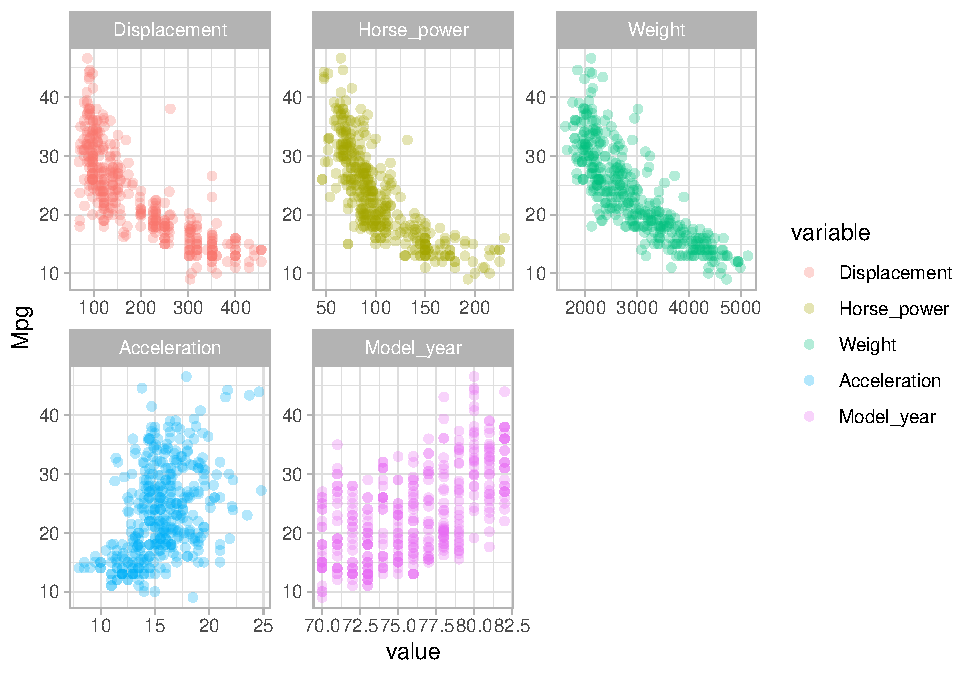
\includegraphics{Regresion_files/figure-latex/unnamed-chunk-2-1} \end{center}

Como dijimos, se aprecia alta correlación entre Displacement,
Horse\_power, Weight respecto de la salida, probablemente de forma
logarítmica.

Las matrices nos correlación nos confirman esta idea (con coeficientes
de Pearson y Kendall)

\begin{Shaded}
\begin{Highlighting}[]
\KeywordTok{corrplot.mixed}\NormalTok{(}\KeywordTok{cor}\NormalTok{(auto), }\DataTypeTok{tl.pos=}\StringTok{"lt"}\NormalTok{, }\DataTypeTok{upper=}\StringTok{"color"}\NormalTok{, }\DataTypeTok{title=}\StringTok{"Pearson"}\NormalTok{)}
\end{Highlighting}
\end{Shaded}

\begin{center}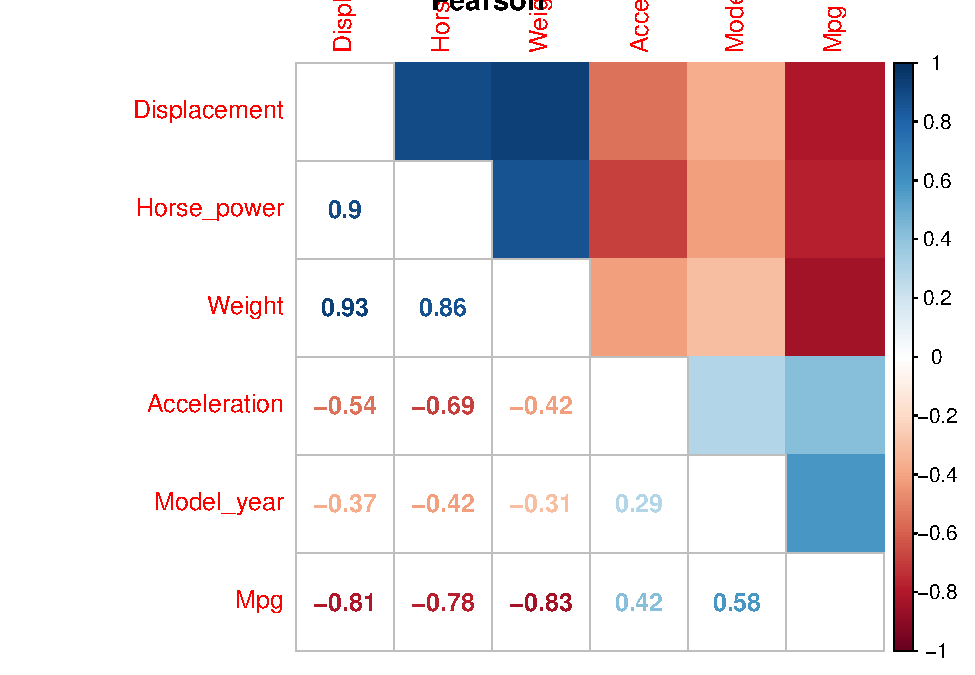
\includegraphics{Regresion_files/figure-latex/unnamed-chunk-3-1} \end{center}

\begin{Shaded}
\begin{Highlighting}[]
\KeywordTok{corrplot.mixed}\NormalTok{(}\KeywordTok{cor}\NormalTok{(auto, }\DataTypeTok{method=}\StringTok{"kendall"}\NormalTok{), }\DataTypeTok{tl.pos=}\StringTok{"lt"}\NormalTok{, }\DataTypeTok{upper=}\StringTok{"color"}\NormalTok{, }\DataTypeTok{title=}\StringTok{"Kendall"}\NormalTok{)}
\end{Highlighting}
\end{Shaded}

\begin{center}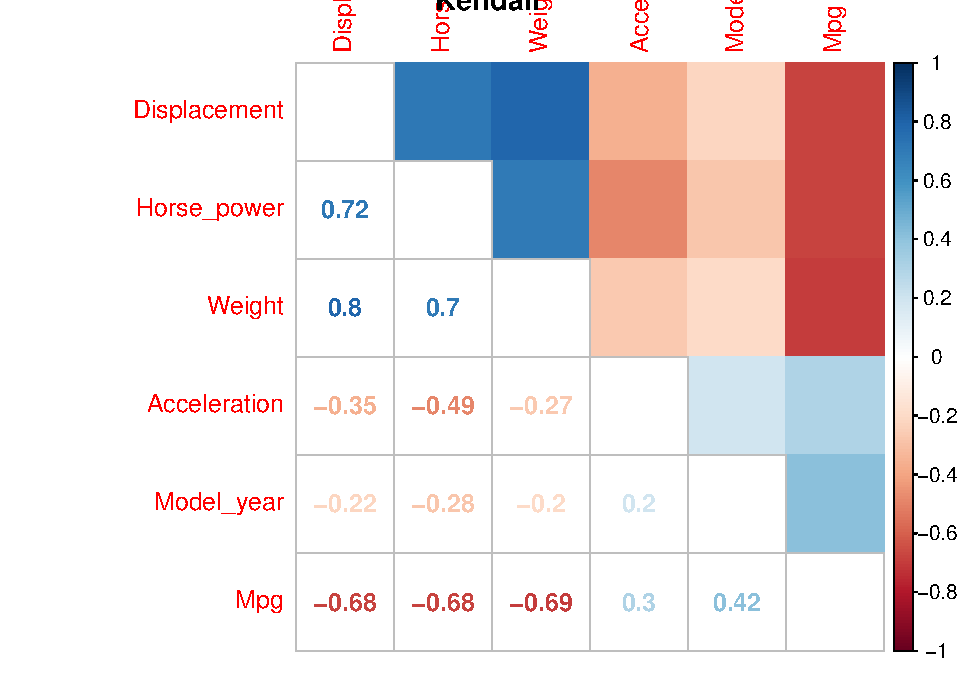
\includegraphics{Regresion_files/figure-latex/unnamed-chunk-3-2} \end{center}

Por tando, si las ordenáramos por cuáles parecen ser más prometedoras,
tendríamos: Weight \textgreater{} Displacement \textgreater{}
Horse\_power \textgreater{} Model\_year \textgreater{} Acceleration

También tenemos que tener en cuenta que las tres primeras variables
están correladas entre sí.

\begin{center}\rule{0.5\linewidth}{0.5pt}\end{center}

\hypertarget{ajustes-de-regresiuxf3n-lineal-univariables}{%
\subsection{Ajustes de regresión lineal
univariables}\label{ajustes-de-regresiuxf3n-lineal-univariables}}

Vamos a analizar un ajuste con cada una de las características:

\begin{Shaded}
\begin{Highlighting}[]
\KeywordTok{lm}\NormalTok{(Mpg }\OperatorTok{~}\StringTok{ }\NormalTok{Weight, }\DataTypeTok{data=}\NormalTok{auto) }\OperatorTok\StringTok{ }\KeywordTok{summary}\NormalTok{()}
\KeywordTok{print}\NormalTok{(}\StringTok{"-------------------------------------------"}\NormalTok{)}
\KeywordTok{lm}\NormalTok{(Mpg }\OperatorTok{~}\StringTok{ }\NormalTok{Displacement, }\DataTypeTok{data=}\NormalTok{auto) }\OperatorTok\StringTok{ }\KeywordTok{summary}\NormalTok{()}
\KeywordTok{print}\NormalTok{(}\StringTok{"-------------------------------------------"}\NormalTok{)}
\KeywordTok{lm}\NormalTok{(Mpg }\OperatorTok{~}\StringTok{ }\NormalTok{Horse_power, }\DataTypeTok{data=}\NormalTok{auto) }\OperatorTok\StringTok{ }\KeywordTok{summary}\NormalTok{()}
\KeywordTok{print}\NormalTok{(}\StringTok{"-------------------------------------------"}\NormalTok{)}
\KeywordTok{lm}\NormalTok{(Mpg }\OperatorTok{~}\StringTok{ }\NormalTok{Model_year, }\DataTypeTok{data=}\NormalTok{auto) }\OperatorTok\StringTok{ }\KeywordTok{summary}\NormalTok{()}
\KeywordTok{print}\NormalTok{(}\StringTok{"-------------------------------------------"}\NormalTok{)}
\KeywordTok{lm}\NormalTok{(Mpg }\OperatorTok{~}\StringTok{ }\NormalTok{Acceleration, }\DataTypeTok{data=}\NormalTok{auto) }\OperatorTok\StringTok{ }\KeywordTok{summary}\NormalTok{()}
\end{Highlighting}
\end{Shaded}

\begin{verbatim}

Call:
lm(formula = Mpg ~ Weight, data = auto)

Residuals:
     Min       1Q   Median       3Q      Max 
-11.9736  -2.7556  -0.3358   2.1379  16.5194 

Coefficients:
             Estimate Std. Error t value Pr(>|t|)    
(Intercept) 46.216524   0.798673   57.87   <2e-16 ***
Weight      -0.007647   0.000258  -29.64   <2e-16 ***
---
Signif. codes:  0 '***' 0.001 '**' 0.01 '*' 0.05 '.' 0.1 ' ' 1

Residual standard error: 4.333 on 390 degrees of freedom
Multiple R-squared:  0.6926,    Adjusted R-squared:  0.6918 
F-statistic: 878.8 on 1 and 390 DF,  p-value: < 2.2e-16

[1] "-------------------------------------------"

Call:
lm(formula = Mpg ~ Displacement, data = auto)

Residuals:
     Min       1Q   Median       3Q      Max 
-12.9170  -3.0243  -0.5021   2.3512  18.6128 

Coefficients:
             Estimate Std. Error t value Pr(>|t|)    
(Intercept)  35.12064    0.49443   71.03   <2e-16 ***
Displacement -0.06005    0.00224  -26.81   <2e-16 ***
---
Signif. codes:  0 '***' 0.001 '**' 0.01 '*' 0.05 '.' 0.1 ' ' 1

Residual standard error: 4.635 on 390 degrees of freedom
Multiple R-squared:  0.6482,    Adjusted R-squared:  0.6473 
F-statistic: 718.7 on 1 and 390 DF,  p-value: < 2.2e-16

[1] "-------------------------------------------"

Call:
lm(formula = Mpg ~ Horse_power, data = auto)

Residuals:
     Min       1Q   Median       3Q      Max 
-13.5710  -3.2592  -0.3435   2.7630  16.9240 

Coefficients:
             Estimate Std. Error t value Pr(>|t|)    
(Intercept) 39.935861   0.717499   55.66   <2e-16 ***
Horse_power -0.157845   0.006446  -24.49   <2e-16 ***
---
Signif. codes:  0 '***' 0.001 '**' 0.01 '*' 0.05 '.' 0.1 ' ' 1

Residual standard error: 4.906 on 390 degrees of freedom
Multiple R-squared:  0.6059,    Adjusted R-squared:  0.6049 
F-statistic: 599.7 on 1 and 390 DF,  p-value: < 2.2e-16

[1] "-------------------------------------------"

Call:
lm(formula = Mpg ~ Model_year, data = auto)

Residuals:
     Min       1Q   Median       3Q      Max 
-12.0212  -5.4411  -0.4412   4.9739  18.2088 

Coefficients:
             Estimate Std. Error t value Pr(>|t|)    
(Intercept) -70.01167    6.64516  -10.54   <2e-16 ***
Model_year    1.23004    0.08736   14.08   <2e-16 ***
---
Signif. codes:  0 '***' 0.001 '**' 0.01 '*' 0.05 '.' 0.1 ' ' 1

Residual standard error: 6.363 on 390 degrees of freedom
Multiple R-squared:  0.337, Adjusted R-squared:  0.3353 
F-statistic: 198.3 on 1 and 390 DF,  p-value: < 2.2e-16

[1] "-------------------------------------------"

Call:
lm(formula = Mpg ~ Acceleration, data = auto)

Residuals:
    Min      1Q  Median      3Q     Max 
-17.989  -5.616  -1.199   4.801  23.239 

Coefficients:
             Estimate Std. Error t value Pr(>|t|)    
(Intercept)    4.8332     2.0485   2.359   0.0188 *  
Acceleration   1.1976     0.1298   9.228   <2e-16 ***
---
Signif. codes:  0 '***' 0.001 '**' 0.01 '*' 0.05 '.' 0.1 ' ' 1

Residual standard error: 7.08 on 390 degrees of freedom
Multiple R-squared:  0.1792,    Adjusted R-squared:  0.1771 
F-statistic: 85.15 on 1 and 390 DF,  p-value: < 2.2e-16
\end{verbatim}

Al ser univariable, no es necesario fijarse en el estadístico F por
ahora. Para ver el potencial de la variable, debemos darle importancia
al p-valor (comprobar de que sea lo suficientemente bajo), y
posteriormente ver el R2 para everiguar el porcentaje de la salida
explicada.

En base a los resultados vemos que el test de correlación nos había
ayudado correctamente: de forma individual todas las variables tienen
dependencia lineal, y el orden de calidad coincide con el orden de
fuerza en las correlaciones.

Guardamos el modelo aditivo hasta ahora

\begin{Shaded}
\begin{Highlighting}[]
\NormalTok{fit <-}\StringTok{ }\KeywordTok{lm}\NormalTok{(Mpg }\OperatorTok{~}\StringTok{ }\NormalTok{Weight, }\DataTypeTok{data=}\NormalTok{auto)}
\end{Highlighting}
\end{Shaded}

Ya con el uso de la variable Weight vemos que podemos explicar un
\textasciitilde69\% de la salida, un buen valor de partida. Graficamos
el ajuste:

\begin{Shaded}
\begin{Highlighting}[]
\KeywordTok{ggplot}\NormalTok{(auto, }\KeywordTok{aes}\NormalTok{(}\DataTypeTok{x=}\NormalTok{Weight, }\DataTypeTok{y=}\NormalTok{Mpg)) }\OperatorTok{+}
\StringTok{  }\KeywordTok{geom_point}\NormalTok{() }\OperatorTok{+}
\StringTok{  }\KeywordTok{geom_smooth}\NormalTok{(}\DataTypeTok{formula =}\NormalTok{ y }\OperatorTok{~}\StringTok{ }\NormalTok{x, }\DataTypeTok{method=}\NormalTok{lm, }\DataTypeTok{col=}\StringTok{"red"}\NormalTok{) }\OperatorTok{+}
\StringTok{  }\KeywordTok{theme_light}\NormalTok{()}
\end{Highlighting}
\end{Shaded}

\begin{center}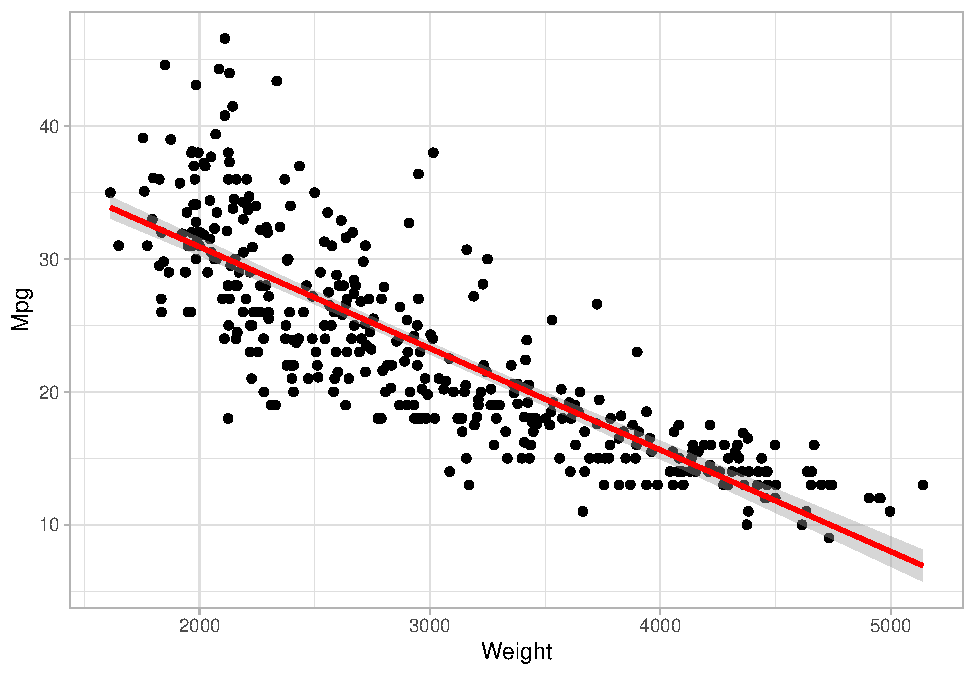
\includegraphics{Regresion_files/figure-latex/unnamed-chunk-6-1} \end{center}

Y vemos sus coeficientes:

\begin{Shaded}
\begin{Highlighting}[]
\KeywordTok{confint}\NormalTok{(fit)}
\end{Highlighting}
\end{Shaded}

\begin{verbatim}
                   2.5 %      97.5 %
(Intercept) 44.646282308 47.78676679
Weight      -0.008154515 -0.00714017
\end{verbatim}

Aunque los valores del intervalo del coeficiente de Weight sea bajo,
vemos que no incluye el cero (y con el p-valor obtenido anteriormente,
lo podemos asegurar con bastante certeza). Probablemente la razón de
estos coeficientes tan pequeños es que los datos no están estandarizados
(se podría hacer perfectamente, se han dejado con sus rangos normales
para interpretarlos mejor) y los valores de las unidades de medida son
bastante diferentes (hablamos de rangos de {[}9.0,46.6{]} en Mpg frente
a {[}1613,5140{]} en Weight)

Ya con esto podemos intentan interpretar un poco los datos, tendríamos
por ahora la fórmula de regresión lineal: (poner fórmula)

(INTERPRETAR ?) La fórmula nos indica que por cada unidad de peso el Mpg
decrementa ?

\begin{center}\rule{0.5\linewidth}{0.5pt}\end{center}

\hypertarget{ajustes-de-regresiuxf3n-lineal-multivariable}{%
\subsection{Ajustes de regresión lineal
multivariable}\label{ajustes-de-regresiuxf3n-lineal-multivariable}}

Aplicamos un método descendente

\begin{Shaded}
\begin{Highlighting}[]
\KeywordTok{lm}\NormalTok{(Mpg }\OperatorTok{~}\StringTok{ }\NormalTok{., }\DataTypeTok{data=}\NormalTok{auto) }\OperatorTok\StringTok{ }\KeywordTok{summary}\NormalTok{()}
\end{Highlighting}
\end{Shaded}

\begin{verbatim}

Call:
lm(formula = Mpg ~ ., data = auto)

Residuals:
    Min      1Q  Median      3Q     Max 
-8.5211 -2.3920 -0.1036  2.0312 14.2874 

Coefficients:
               Estimate Std. Error t value Pr(>|t|)    
(Intercept)  -1.544e+01  4.677e+00  -3.300  0.00106 ** 
Displacement  2.782e-03  5.462e-03   0.509  0.61082    
Horse_power   1.020e-03  1.376e-02   0.074  0.94095    
Weight       -6.874e-03  6.653e-04 -10.333  < 2e-16 ***
Acceleration  9.032e-02  1.019e-01   0.886  0.37599    
Model_year    7.541e-01  5.261e-02  14.334  < 2e-16 ***
---
Signif. codes:  0 '***' 0.001 '**' 0.01 '*' 0.05 '.' 0.1 ' ' 1

Residual standard error: 3.435 on 386 degrees of freedom
Multiple R-squared:  0.8088,    Adjusted R-squared:  0.8063 
F-statistic: 326.5 on 5 and 386 DF,  p-value: < 2.2e-16
\end{verbatim}

El p-valor del F estadístico nos dice que al menos hay una variable
(realmente ya lo sabíamos de los ajustes univariables) con dependencia
linea.

Vemos que hay 3 variables con mal p-valor, empezamos quitando la que lo
tiene más alto, Horse\_power

\begin{Shaded}
\begin{Highlighting}[]
\KeywordTok{lm}\NormalTok{(Mpg }\OperatorTok{~}\StringTok{ }\NormalTok{. }\OperatorTok{-}\StringTok{ }\NormalTok{Horse_power, }\DataTypeTok{data=}\NormalTok{auto) }\OperatorTok\StringTok{ }\KeywordTok{summary}\NormalTok{()}
\end{Highlighting}
\end{Shaded}

\begin{verbatim}

Call:
lm(formula = Mpg ~ . - Horse_power, data = auto)

Residuals:
    Min      1Q  Median      3Q     Max 
-8.5182 -2.3948 -0.1085  2.0405 14.2908 

Coefficients:
               Estimate Std. Error t value Pr(>|t|)    
(Intercept)  -1.527e+01  4.106e+00  -3.719 0.000229 ***
Displacement  2.874e-03  5.310e-03   0.541 0.588651    
Weight       -6.852e-03  5.967e-04 -11.483  < 2e-16 ***
Acceleration  8.555e-02  7.885e-02   1.085 0.278595    
Model_year    7.532e-01  5.118e-02  14.717  < 2e-16 ***
---
Signif. codes:  0 '***' 0.001 '**' 0.01 '*' 0.05 '.' 0.1 ' ' 1

Residual standard error: 3.431 on 387 degrees of freedom
Multiple R-squared:  0.8088,    Adjusted R-squared:  0.8068 
F-statistic: 409.2 on 4 and 387 DF,  p-value: < 2.2e-16
\end{verbatim}

El F estadístico está correcto, y seguimos teniendo variables con
p-valor grande, quitamos Displacement

\begin{Shaded}
\begin{Highlighting}[]
\KeywordTok{lm}\NormalTok{(Mpg }\OperatorTok{~}\StringTok{ }\NormalTok{. }\OperatorTok{-}\StringTok{ }\NormalTok{Horse_power }\OperatorTok{-}\StringTok{ }\NormalTok{Displacement, }\DataTypeTok{data=}\NormalTok{auto) }\OperatorTok\StringTok{ }\KeywordTok{summary}\NormalTok{()}
\end{Highlighting}
\end{Shaded}

\begin{verbatim}

Call:
lm(formula = Mpg ~ . - Horse_power - Displacement, data = auto)

Residuals:
    Min      1Q  Median      3Q     Max 
-8.6749 -2.3528 -0.1082  2.0168 14.3022 

Coefficients:
               Estimate Std. Error t value Pr(>|t|)    
(Intercept)  -14.936555   4.055512  -3.683 0.000263 ***
Weight        -0.006554   0.000230 -28.502  < 2e-16 ***
Acceleration   0.066359   0.070361   0.943 0.346204    
Model_year     0.748446   0.050366  14.860  < 2e-16 ***
---
Signif. codes:  0 '***' 0.001 '**' 0.01 '*' 0.05 '.' 0.1 ' ' 1

Residual standard error: 3.428 on 388 degrees of freedom
Multiple R-squared:  0.8086,    Adjusted R-squared:  0.8071 
F-statistic: 546.5 on 3 and 388 DF,  p-value: < 2.2e-16
\end{verbatim}

idem. a lo anterior, quitamos Acceleration.

\begin{Shaded}
\begin{Highlighting}[]
\KeywordTok{lm}\NormalTok{(Mpg }\OperatorTok{~}\StringTok{ }\NormalTok{. }\OperatorTok{-}\StringTok{ }\NormalTok{Horse_power }\OperatorTok{-}\StringTok{ }\NormalTok{Displacement }\OperatorTok{-}\StringTok{ }\NormalTok{Acceleration, }\DataTypeTok{data=}\NormalTok{auto) }\OperatorTok\StringTok{ }\KeywordTok{summary}\NormalTok{()}
\end{Highlighting}
\end{Shaded}

\begin{verbatim}

Call:
lm(formula = Mpg ~ . - Horse_power - Displacement - Acceleration, 
    data = auto)

Residuals:
    Min      1Q  Median      3Q     Max 
-8.8505 -2.3014 -0.1167  2.0367 14.3555 

Coefficients:
              Estimate Std. Error t value Pr(>|t|)    
(Intercept) -1.435e+01  4.007e+00  -3.581 0.000386 ***
Weight      -6.632e-03  2.146e-04 -30.911  < 2e-16 ***
Model_year   7.573e-01  4.947e-02  15.308  < 2e-16 ***
---
Signif. codes:  0 '***' 0.001 '**' 0.01 '*' 0.05 '.' 0.1 ' ' 1

Residual standard error: 3.427 on 389 degrees of freedom
Multiple R-squared:  0.8082,    Adjusted R-squared:  0.8072 
F-statistic: 819.5 on 2 and 389 DF,  p-value: < 2.2e-16
\end{verbatim}

El estadístico F sigue bien, y los p-valores de las variables son
extremadamente bajos. Nos fijamos en el R2 y vemos que ha subido
considerablemente (un 10\%) respecto al univariable, por lo que este
sería nuestro modelo aditivo por ahora.

A partir de ahora hay que tener cuidado si el R2 sigue aumentando, hay
que evitar el overfitting en el modelo.

\begin{center}\rule{0.5\linewidth}{0.5pt}\end{center}

\hypertarget{inserciuxf3n-de-interacciones}{%
\subsection{Inserción de
interacciones}\label{inserciuxf3n-de-interacciones}}

Del modelo aditivo solo nos han quedado dos regresores, así que probamos
a incluirlos como interacción.

\begin{Shaded}
\begin{Highlighting}[]
\KeywordTok{lm}\NormalTok{(Mpg }\OperatorTok{~}\StringTok{ }\OperatorTok{+}\StringTok{ }\NormalTok{Weight }\OperatorTok{*}\StringTok{ }\NormalTok{Model_year, }\DataTypeTok{data=}\NormalTok{auto) }\OperatorTok\StringTok{ }\KeywordTok{summary}\NormalTok{()}
\end{Highlighting}
\end{Shaded}

\begin{verbatim}

Call:
lm(formula = Mpg ~ +Weight * Model_year, data = auto)

Residuals:
    Min      1Q  Median      3Q     Max 
-8.0397 -1.9956 -0.0983  1.6525 12.9896 

Coefficients:
                    Estimate Std. Error t value Pr(>|t|)    
(Intercept)       -1.105e+02  1.295e+01  -8.531 3.30e-16 ***
Weight             2.755e-02  4.413e-03   6.242 1.14e-09 ***
Model_year         2.040e+00  1.718e-01  11.876  < 2e-16 ***
Weight:Model_year -4.579e-04  5.907e-05  -7.752 8.02e-14 ***
---
Signif. codes:  0 '***' 0.001 '**' 0.01 '*' 0.05 '.' 0.1 ' ' 1

Residual standard error: 3.193 on 388 degrees of freedom
Multiple R-squared:  0.8339,    Adjusted R-squared:  0.8326 
F-statistic: 649.3 on 3 and 388 DF,  p-value: < 2.2e-16
\end{verbatim}

El F estadístico sigue bien y los p-valores son bajos, el nuevo R2 ha
mejorado un 3\%, así que no es demasiado para considerar un overfitting.
Probablemente más de un 90\% sería preocupante, pero también tenemos que
tener en cuenta que las variables están fuertemente correladas con la
salida.

Podríamos probar a añadir alguna interacción más con alguna variable que
no hubiera entrado en el modelo aditivo, pero no se espera que mejore:

\begin{Shaded}
\begin{Highlighting}[]
\KeywordTok{lm}\NormalTok{(Mpg }\OperatorTok{~}\StringTok{ }\OperatorTok{+}\StringTok{ }\NormalTok{Weight }\OperatorTok{*}\StringTok{ }\NormalTok{Model_year }\OperatorTok{+}\StringTok{ }\NormalTok{Acceleration }\OperatorTok{*}\StringTok{ }\NormalTok{Displacement, }\DataTypeTok{data=}\NormalTok{auto) }\OperatorTok\StringTok{ }\KeywordTok{summary}\NormalTok{()}
\end{Highlighting}
\end{Shaded}

\begin{verbatim}

Call:
lm(formula = Mpg ~ +Weight * Model_year + Acceleration * Displacement, 
    data = auto)

Residuals:
    Min      1Q  Median      3Q     Max 
-7.3130 -1.8670 -0.0426  1.6109 12.2499 

Coefficients:
                            Estimate Std. Error t value Pr(>|t|)    
(Intercept)               -1.131e+02  1.321e+01  -8.564 2.65e-16 ***
Weight                     2.456e-02  4.693e-03   5.234 2.73e-07 ***
Model_year                 1.907e+00  1.769e-01  10.778  < 2e-16 ***
Acceleration               7.273e-01  1.282e-01   5.671 2.79e-08 ***
Displacement               3.605e-02  8.673e-03   4.157 3.98e-05 ***
Weight:Model_year         -4.054e-04  6.281e-05  -6.454 3.29e-10 ***
Acceleration:Displacement -2.953e-03  6.219e-04  -4.748 2.91e-06 ***
---
Signif. codes:  0 '***' 0.001 '**' 0.01 '*' 0.05 '.' 0.1 ' ' 1

Residual standard error: 3.075 on 385 degrees of freedom
Multiple R-squared:  0.8472,    Adjusted R-squared:  0.8448 
F-statistic: 355.7 on 6 and 385 DF,  p-value: < 2.2e-16
\end{verbatim}

A pesar de nuestra suposición los p-valores son válidos y el R2 aumenta
un 1\%. Es cuestionable si el aumento de la complejidad del modelo
merece con este incremento de R2. Por simplificar vamos a quedarnos con
el modelo aditivo anterior y probar con otra interacción.

Podemos probar combinando la variable Acceleration con una de que
teníamos (Weight y Model\_year)

\begin{Shaded}
\begin{Highlighting}[]
\KeywordTok{lm}\NormalTok{(Mpg }\OperatorTok{~}\StringTok{ }\OperatorTok{+}\StringTok{ }\NormalTok{Weight }\OperatorTok{*}\StringTok{ }\NormalTok{Model_year }\OperatorTok{+}\StringTok{ }\NormalTok{Acceleration }\OperatorTok{*}\StringTok{ }\NormalTok{Weight, }\DataTypeTok{data=}\NormalTok{auto) }\OperatorTok\StringTok{ }\KeywordTok{summary}\NormalTok{()}
\end{Highlighting}
\end{Shaded}

\begin{verbatim}

Call:
lm(formula = Mpg ~ +Weight * Model_year + Acceleration * Weight, 
    data = auto)

Residuals:
    Min      1Q  Median      3Q     Max 
-7.4473 -1.7994 -0.0496  1.4790 12.1258 

Coefficients:
                      Estimate Std. Error t value Pr(>|t|)    
(Intercept)         -1.230e+02  1.298e+01  -9.480  < 2e-16 ***
Weight               2.971e-02  4.419e-03   6.722 6.47e-11 ***
Model_year           1.926e+00  1.742e-01  11.055  < 2e-16 ***
Acceleration         1.341e+00  2.323e-01   5.772 1.61e-08 ***
Weight:Model_year   -4.078e-04  6.197e-05  -6.581 1.53e-10 ***
Weight:Acceleration -3.808e-04  7.537e-05  -5.052 6.76e-07 ***
---
Signif. codes:  0 '***' 0.001 '**' 0.01 '*' 0.05 '.' 0.1 ' ' 1

Residual standard error: 3.061 on 386 degrees of freedom
Multiple R-squared:  0.8482,    Adjusted R-squared:  0.8462 
F-statistic: 431.4 on 5 and 386 DF,  p-value: < 2.2e-16
\end{verbatim}

\begin{Shaded}
\begin{Highlighting}[]
\KeywordTok{lm}\NormalTok{(Mpg }\OperatorTok{~}\StringTok{ }\OperatorTok{+}\StringTok{ }\NormalTok{Weight }\OperatorTok{*}\StringTok{ }\NormalTok{Model_year }\OperatorTok{+}\StringTok{ }\NormalTok{Acceleration }\OperatorTok{*}\StringTok{ }\NormalTok{Model_year, }\DataTypeTok{data=}\NormalTok{auto) }\OperatorTok\StringTok{ }\KeywordTok{summary}\NormalTok{()}
\end{Highlighting}
\end{Shaded}

\begin{verbatim}

Call:
lm(formula = Mpg ~ +Weight * Model_year + Acceleration * Model_year, 
    data = auto)

Residuals:
    Min      1Q  Median      3Q     Max 
-7.8674 -1.9539 -0.0617  1.7397 12.3964 

Coefficients:
                          Estimate Std. Error t value Pr(>|t|)    
(Intercept)             -4.046e+01  2.833e+01  -1.428  0.15401    
Weight                   2.523e-02  4.881e-03   5.170 3.76e-07 ***
Model_year               1.072e+00  3.704e-01   2.895  0.00401 ** 
Acceleration            -3.956e+00  1.268e+00  -3.120  0.00195 ** 
Weight:Model_year       -4.263e-04  6.475e-05  -6.584 1.49e-10 ***
Model_year:Acceleration  5.476e-02  1.663e-02   3.293  0.00108 ** 
---
Signif. codes:  0 '***' 0.001 '**' 0.01 '*' 0.05 '.' 0.1 ' ' 1

Residual standard error: 3.117 on 386 degrees of freedom
Multiple R-squared:  0.8426,    Adjusted R-squared:  0.8406 
F-statistic: 413.2 on 5 and 386 DF,  p-value: < 2.2e-16
\end{verbatim}

Y entre los dos nos podríamos quedar con el primero por tener mejores
p-valores y un mejor R2. Aun así, el incremento es pequeño respecto a
nuestro modelo aditivo.

La fórmula del modelo aditivo que llevamos por ahora es:

Y la graficamos:

\begin{Shaded}
\begin{Highlighting}[]
\NormalTok{fit <-}\StringTok{ }\KeywordTok{lm}\NormalTok{(Mpg }\OperatorTok{~}\StringTok{ }\NormalTok{Weight }\OperatorTok{*}\StringTok{ }\NormalTok{Model_year }\OperatorTok{+}\StringTok{ }\NormalTok{Acceleration }\OperatorTok{*}\StringTok{ }\NormalTok{Weight, }\DataTypeTok{data=}\NormalTok{auto)}

\NormalTok{predicted_df <-}\StringTok{ }\KeywordTok{data.frame}\NormalTok{(}\DataTypeTok{mpg_pred =} \KeywordTok{predict}\NormalTok{(fit, auto), }\DataTypeTok{hp=}\NormalTok{auto}\OperatorTok{$}\NormalTok{Weight)}

\CommentTok{# this is the predicted line of multiple linear regression}
\KeywordTok{ggplot}\NormalTok{(}\DataTypeTok{data =}\NormalTok{ auto, }\KeywordTok{aes}\NormalTok{(}\DataTypeTok{y =}\NormalTok{ Mpg, }\DataTypeTok{x =}\NormalTok{ Weight)) }\OperatorTok{+}\StringTok{ }
\StringTok{  }\KeywordTok{geom_point}\NormalTok{() }\OperatorTok{+}
\StringTok{  }\KeywordTok{geom_line}\NormalTok{(}\DataTypeTok{color=}\StringTok{'red'}\NormalTok{, }\DataTypeTok{data =}\NormalTok{ predicted_df, }\KeywordTok{aes}\NormalTok{(}\DataTypeTok{y=}\NormalTok{mpg_pred, }\DataTypeTok{x=}\NormalTok{hp)) }\OperatorTok{+}
\StringTok{  }\KeywordTok{theme_light}\NormalTok{()}
\end{Highlighting}
\end{Shaded}

\begin{center}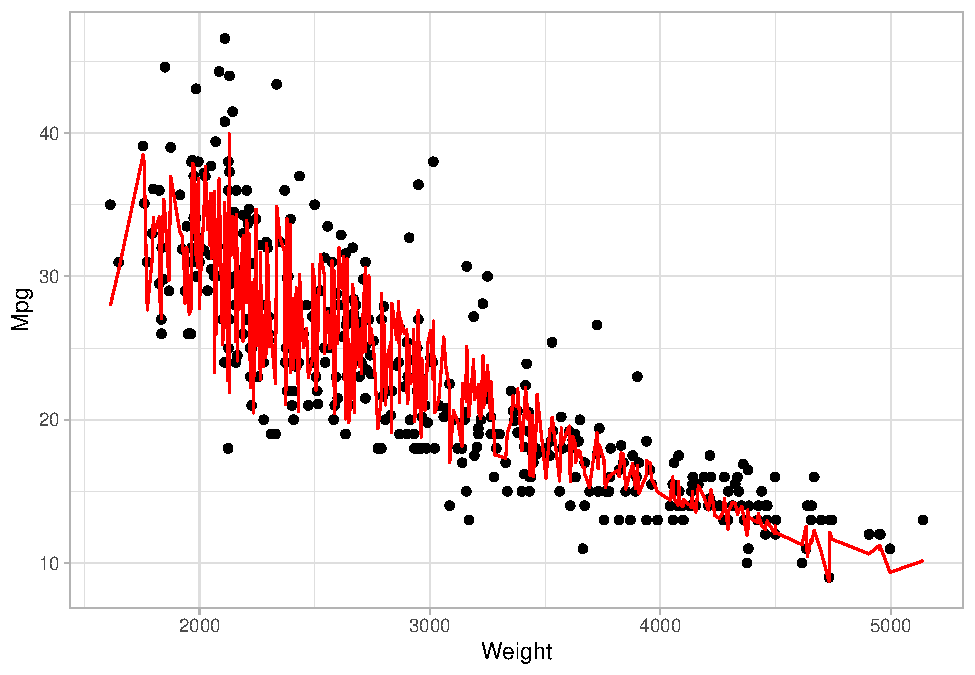
\includegraphics{Regresion_files/figure-latex/unnamed-chunk-16-1} \end{center}

Se aprecia posible overfitting en el modelo, vamos a dejarlo por ahora e
intentar solucionarlo con el modelo no lineal.

\begin{center}\rule{0.5\linewidth}{0.5pt}\end{center}

\hypertarget{ajustes-de-regresiuxf3n-no-lineal}{%
\subsection{Ajustes de regresión no
lineal}\label{ajustes-de-regresiuxf3n-no-lineal}}

Habíamos dicho que las gráficas nos mostraban una tendencia logarítmica,
vamos a incluír la de Weight en nuestro modelo aditivo

\begin{Shaded}
\begin{Highlighting}[]
\KeywordTok{lm}\NormalTok{(Mpg }\OperatorTok{~}\StringTok{ }\OperatorTok{+}\StringTok{ }\NormalTok{Weight }\OperatorTok{*}\StringTok{ }\NormalTok{Model_year }\OperatorTok{+}\StringTok{ }\NormalTok{Acceleration }\OperatorTok{*}\StringTok{ }\NormalTok{Weight }\OperatorTok{+}\StringTok{ }\KeywordTok{I}\NormalTok{(}\KeywordTok{log}\NormalTok{(Weight)), }\DataTypeTok{data=}\NormalTok{auto) }\OperatorTok\StringTok{ }
\StringTok{  }\KeywordTok{summary}\NormalTok{()}
\end{Highlighting}
\end{Shaded}

\begin{verbatim}

Call:
lm(formula = Mpg ~ +Weight * Model_year + Acceleration * Weight + 
    I(log(Weight)), data = auto)

Residuals:
    Min      1Q  Median      3Q     Max 
-7.6734 -1.7933 -0.0576  1.3154 12.1716 

Coefficients:
                      Estimate Std. Error t value Pr(>|t|)    
(Intercept)          1.191e+02  4.120e+01   2.891  0.00406 ** 
Weight               2.842e-02  4.227e-03   6.723 6.44e-11 ***
Model_year           1.638e+00  1.728e-01   9.480  < 2e-16 ***
Acceleration         7.236e-01  2.435e-01   2.972  0.00315 ** 
I(log(Weight))      -3.028e+01  4.914e+00  -6.162 1.81e-09 ***
Weight:Model_year   -2.971e-04  6.186e-05  -4.803 2.24e-06 ***
Weight:Acceleration -1.775e-04  7.919e-05  -2.241  0.02559 *  
---
Signif. codes:  0 '***' 0.001 '**' 0.01 '*' 0.05 '.' 0.1 ' ' 1

Residual standard error: 2.924 on 385 degrees of freedom
Multiple R-squared:  0.8618,    Adjusted R-squared:  0.8597 
F-statistic: 400.2 on 6 and 385 DF,  p-value: < 2.2e-16
\end{verbatim}

El estadístico F está bien y los p-valores también, aunque el de la
interacción Weight-Acceleration es alto comparado con el resto (aún así
sigue siendo aceptable).

Como el R2 ha subido, por ver si mejora, vamos a quitar esta
interacción.

\begin{Shaded}
\begin{Highlighting}[]
\KeywordTok{lm}\NormalTok{(Mpg }\OperatorTok{~}\StringTok{ }\OperatorTok{+}\StringTok{ }\NormalTok{Weight }\OperatorTok{*}\StringTok{ }\NormalTok{Model_year }\OperatorTok{+}\StringTok{ }\KeywordTok{I}\NormalTok{(}\KeywordTok{log}\NormalTok{(Weight)), }\DataTypeTok{data=}\NormalTok{auto) }\OperatorTok\StringTok{ }
\StringTok{  }\KeywordTok{summary}\NormalTok{()}
\end{Highlighting}
\end{Shaded}

\begin{verbatim}

Call:
lm(formula = Mpg ~ +Weight * Model_year + I(log(Weight)), data = auto)

Residuals:
    Min      1Q  Median      3Q     Max 
-8.7501 -1.7470 -0.0725  1.3122 12.6776 

Coefficients:
                    Estimate Std. Error t value Pr(>|t|)    
(Intercept)        1.715e+02  3.810e+01   4.501 8.98e-06 ***
Weight             2.522e-02  4.119e-03   6.123 2.25e-09 ***
Model_year         1.572e+00  1.708e-01   9.202  < 2e-16 ***
I(log(Weight))    -3.540e+01  4.538e+00  -7.800 5.82e-14 ***
Weight:Model_year -2.701e-04  6.003e-05  -4.499 9.04e-06 ***
---
Signif. codes:  0 '***' 0.001 '**' 0.01 '*' 0.05 '.' 0.1 ' ' 1

Residual standard error: 2.972 on 387 degrees of freedom
Multiple R-squared:  0.8565,    Adjusted R-squared:  0.855 
F-statistic: 577.3 on 4 and 387 DF,  p-value: < 2.2e-16
\end{verbatim}

Hemos empeorado un 0.5\%, bastante poco, y el modelo es más simple. La
dejamos quitada.

Podemos mostrarlo en un gráfico:

\begin{Shaded}
\begin{Highlighting}[]
\NormalTok{fit <-}\StringTok{ }\KeywordTok{lm}\NormalTok{(Mpg }\OperatorTok{~}\StringTok{ }\OperatorTok{+}\StringTok{ }\NormalTok{Weight }\OperatorTok{*}\StringTok{ }\NormalTok{Model_year }\OperatorTok{+}\StringTok{ }\KeywordTok{I}\NormalTok{(}\KeywordTok{log}\NormalTok{(Weight)), }\DataTypeTok{data=}\NormalTok{auto)}

\NormalTok{predicted_df <-}\StringTok{ }\KeywordTok{data.frame}\NormalTok{(}\DataTypeTok{mpg_pred =} \KeywordTok{predict}\NormalTok{(fit, auto), }\DataTypeTok{hp=}\NormalTok{auto}\OperatorTok{$}\NormalTok{Weight)}

\CommentTok{# this is the predicted line of multiple linear regression}
\KeywordTok{ggplot}\NormalTok{(}\DataTypeTok{data =}\NormalTok{ auto, }\KeywordTok{aes}\NormalTok{(}\DataTypeTok{y =}\NormalTok{ Mpg, }\DataTypeTok{x =}\NormalTok{ Weight)) }\OperatorTok{+}\StringTok{ }
\StringTok{  }\KeywordTok{geom_point}\NormalTok{() }\OperatorTok{+}
\StringTok{  }\KeywordTok{geom_line}\NormalTok{(}\DataTypeTok{color=}\StringTok{'red'}\NormalTok{, }\DataTypeTok{data =}\NormalTok{ predicted_df, }\KeywordTok{aes}\NormalTok{(}\DataTypeTok{y=}\NormalTok{mpg_pred, }\DataTypeTok{x=}\NormalTok{hp)) }\OperatorTok{+}
\StringTok{  }\KeywordTok{theme_light}\NormalTok{()}
\end{Highlighting}
\end{Shaded}

\begin{center}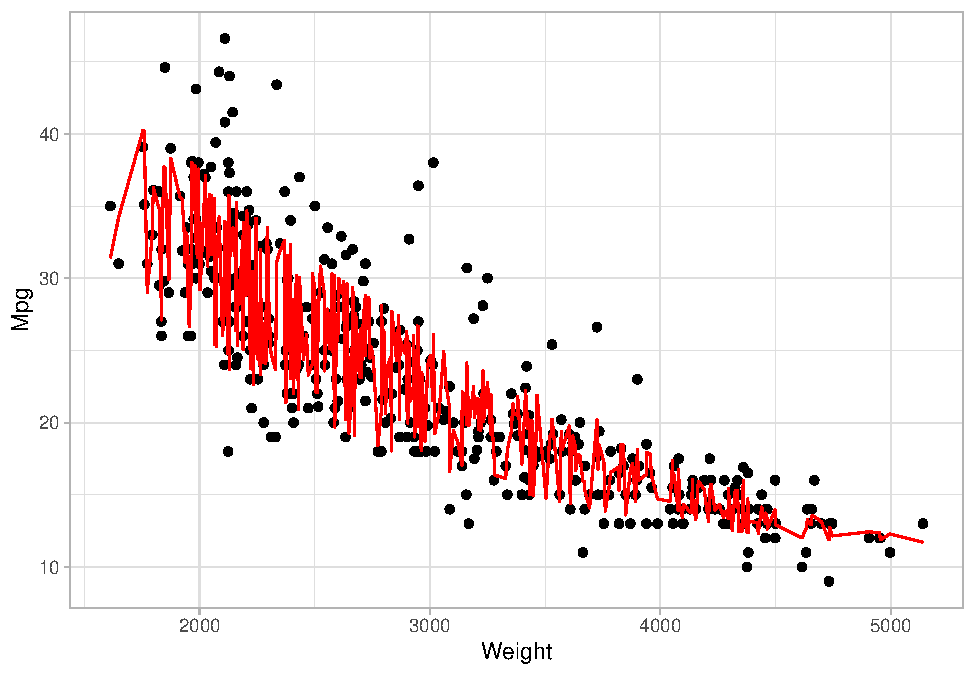
\includegraphics{Regresion_files/figure-latex/unnamed-chunk-19-1} \end{center}

Esta gráfica nos indica que con casi toda probabilidad se está generando
sobreajuste, se ve necesario simplificar el modelo.

Si quitamos la otra interacción:

\begin{Shaded}
\begin{Highlighting}[]
\KeywordTok{lm}\NormalTok{(Mpg }\OperatorTok{~}\StringTok{ }\NormalTok{Weight }\OperatorTok{+}\StringTok{ }\NormalTok{Model_year }\OperatorTok{+}\StringTok{ }\KeywordTok{I}\NormalTok{(}\KeywordTok{log}\NormalTok{(Weight)), }\DataTypeTok{data=}\NormalTok{auto) }\OperatorTok\StringTok{ }\KeywordTok{summary}\NormalTok{()}
\end{Highlighting}
\end{Shaded}

\begin{verbatim}

Call:
lm(formula = Mpg ~ Weight + Model_year + I(log(Weight)), data = auto)

Residuals:
    Min      1Q  Median      3Q     Max 
-9.3384 -1.7476 -0.2122  1.5322 13.2812 

Coefficients:
                 Estimate Std. Error t value Pr(>|t|)    
(Intercept)    284.287315  29.392946   9.672  < 2e-16 ***
Weight           0.007772   0.001420   5.473 7.97e-08 ***
Model_year       0.828693   0.044506  18.620  < 2e-16 ***
I(log(Weight)) -43.590633   4.258803 -10.235  < 2e-16 ***
---
Signif. codes:  0 '***' 0.001 '**' 0.01 '*' 0.05 '.' 0.1 ' ' 1

Residual standard error: 3.045 on 388 degrees of freedom
Multiple R-squared:  0.849, Adjusted R-squared:  0.8478 
F-statistic:   727 on 3 and 388 DF,  p-value: < 2.2e-16
\end{verbatim}

No hemos perdido apenas R2, mostramos la gráfica:

\begin{Shaded}
\begin{Highlighting}[]
\NormalTok{fit <-}\StringTok{ }\KeywordTok{lm}\NormalTok{(Mpg }\OperatorTok{~}\StringTok{ }\NormalTok{Weight }\OperatorTok{+}\StringTok{ }\NormalTok{Model_year}\OperatorTok{+}\StringTok{ }\KeywordTok{I}\NormalTok{(}\KeywordTok{log}\NormalTok{(Weight)), }\DataTypeTok{data=}\NormalTok{auto)}

\NormalTok{predicted_df <-}\StringTok{ }\KeywordTok{data.frame}\NormalTok{(}\DataTypeTok{mpg_pred =} \KeywordTok{predict}\NormalTok{(fit, auto), }\DataTypeTok{hp=}\NormalTok{auto}\OperatorTok{$}\NormalTok{Weight)}

\CommentTok{# this is the predicted line of multiple linear regression}
\KeywordTok{ggplot}\NormalTok{(}\DataTypeTok{data =}\NormalTok{ auto, }\KeywordTok{aes}\NormalTok{(}\DataTypeTok{y =}\NormalTok{ Mpg, }\DataTypeTok{x =}\NormalTok{ Weight)) }\OperatorTok{+}\StringTok{ }
\StringTok{  }\KeywordTok{geom_point}\NormalTok{() }\OperatorTok{+}
\StringTok{  }\KeywordTok{geom_line}\NormalTok{(}\DataTypeTok{color=}\StringTok{'red'}\NormalTok{, }\DataTypeTok{data =}\NormalTok{ predicted_df, }\KeywordTok{aes}\NormalTok{(}\DataTypeTok{y=}\NormalTok{mpg_pred, }\DataTypeTok{x=}\NormalTok{hp)) }\OperatorTok{+}
\StringTok{  }\KeywordTok{theme_light}\NormalTok{()}
\end{Highlighting}
\end{Shaded}

\begin{center}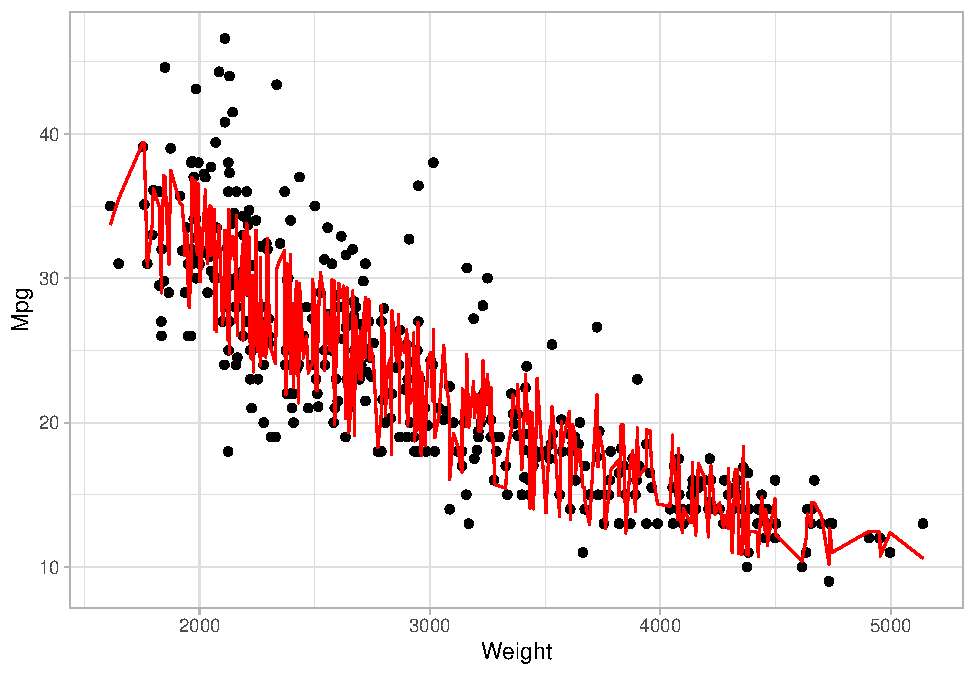
\includegraphics{Regresion_files/figure-latex/unnamed-chunk-21-1} \end{center}

Seguimos con el mismo problema, probablemente se deba a una de las
variables. Quitamos Model\_year por tener poca correlación con la
variable de salida:

\begin{Shaded}
\begin{Highlighting}[]
\KeywordTok{lm}\NormalTok{(Mpg }\OperatorTok{~}\StringTok{ }\NormalTok{Weight }\OperatorTok{+}\StringTok{ }\KeywordTok{I}\NormalTok{(}\KeywordTok{log}\NormalTok{(Weight)), }\DataTypeTok{data=}\NormalTok{auto) }\OperatorTok\StringTok{ }\KeywordTok{summary}\NormalTok{()}
\end{Highlighting}
\end{Shaded}

\begin{verbatim}

Call:
lm(formula = Mpg ~ Weight + I(log(Weight)), data = auto)

Residuals:
     Min       1Q   Median       3Q      Max 
-12.5329  -2.7031  -0.4016   1.7038  16.0835 

Coefficients:
                 Estimate Std. Error t value Pr(>|t|)    
(Intercept)    263.812407  40.366256   6.535 1.99e-10 ***
Weight           0.002582   0.001914   1.349    0.178    
I(log(Weight)) -31.166013   5.780558  -5.392 1.21e-07 ***
---
Signif. codes:  0 '***' 0.001 '**' 0.01 '*' 0.05 '.' 0.1 ' ' 1

Residual standard error: 4.185 on 389 degrees of freedom
Multiple R-squared:  0.714, Adjusted R-squared:  0.7125 
F-statistic: 485.6 on 2 and 389 DF,  p-value: < 2.2e-16
\end{verbatim}

El p-valor de Weight nos indica que hay que quitarla, y al no estar
incluída ninguna interacción, no es un término de jerarquía, por lo que
podemos hacerlo. Se puede porque la variable sigue siendo independiente,
solamente no está modelada de forma lineal, sino logarítmicamente.

\begin{Shaded}
\begin{Highlighting}[]
\KeywordTok{lm}\NormalTok{(Mpg }\OperatorTok{~}\StringTok{ }\KeywordTok{I}\NormalTok{(}\KeywordTok{log}\NormalTok{(Weight)), }\DataTypeTok{data=}\NormalTok{auto) }\OperatorTok\StringTok{ }\KeywordTok{summary}\NormalTok{()}
\end{Highlighting}
\end{Shaded}

\begin{verbatim}

Call:
lm(formula = Mpg ~ I(log(Weight)), data = auto)

Residuals:
     Min       1Q   Median       3Q      Max 
-12.4315  -2.6752  -0.2888   1.9429  16.0136 

Coefficients:
               Estimate Std. Error t value Pr(>|t|)    
(Intercept)    209.9433     6.0002   34.99   <2e-16 ***
I(log(Weight)) -23.4317     0.7534  -31.10   <2e-16 ***
---
Signif. codes:  0 '***' 0.001 '**' 0.01 '*' 0.05 '.' 0.1 ' ' 1

Residual standard error: 4.189 on 390 degrees of freedom
Multiple R-squared:  0.7127,    Adjusted R-squared:  0.7119 
F-statistic: 967.3 on 1 and 390 DF,  p-value: < 2.2e-16
\end{verbatim}

\begin{Shaded}
\begin{Highlighting}[]
\NormalTok{fit <-}\StringTok{ }\KeywordTok{lm}\NormalTok{(Mpg }\OperatorTok{~}\StringTok{ }\KeywordTok{I}\NormalTok{(}\KeywordTok{log}\NormalTok{(Weight)), }\DataTypeTok{data=}\NormalTok{auto)}

\NormalTok{predicted_df <-}\StringTok{ }\KeywordTok{data.frame}\NormalTok{(}\DataTypeTok{mpg_pred =} \KeywordTok{predict}\NormalTok{(fit, auto), }\DataTypeTok{hp=}\NormalTok{auto}\OperatorTok{$}\NormalTok{Weight)}

\CommentTok{# this is the predicted line of multiple linear regression}
\KeywordTok{ggplot}\NormalTok{(}\DataTypeTok{data =}\NormalTok{ auto, }\KeywordTok{aes}\NormalTok{(}\DataTypeTok{y =}\NormalTok{ Mpg, }\DataTypeTok{x =}\NormalTok{ Weight)) }\OperatorTok{+}\StringTok{ }
\StringTok{  }\KeywordTok{geom_point}\NormalTok{() }\OperatorTok{+}
\StringTok{  }\KeywordTok{geom_line}\NormalTok{(}\DataTypeTok{color=}\StringTok{'red'}\NormalTok{, }\DataTypeTok{data =}\NormalTok{ predicted_df, }\KeywordTok{aes}\NormalTok{(}\DataTypeTok{y=}\NormalTok{mpg_pred, }\DataTypeTok{x=}\NormalTok{hp)) }\OperatorTok{+}
\StringTok{  }\KeywordTok{theme_light}\NormalTok{()}
\end{Highlighting}
\end{Shaded}

\begin{center}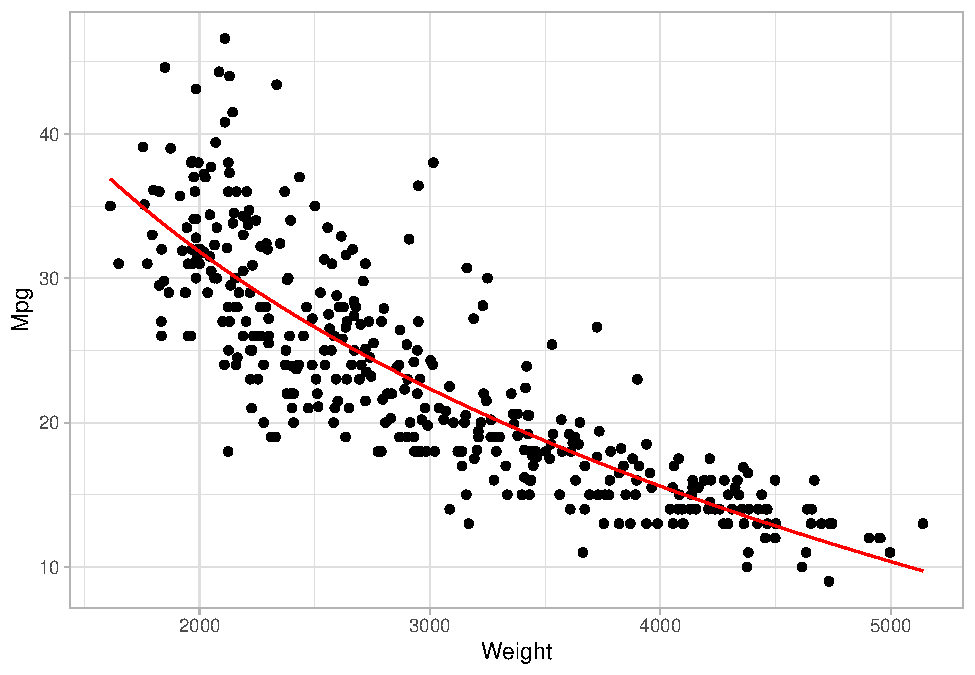
\includegraphics{Regresion_files/figure-latex/unnamed-chunk-24-1} \end{center}

\begin{Shaded}
\begin{Highlighting}[]
\NormalTok{predicted_df <-}\StringTok{ }\KeywordTok{data.frame}\NormalTok{(}\DataTypeTok{mpg_pred =} \KeywordTok{predict}\NormalTok{(fit, auto), }\DataTypeTok{hp=}\NormalTok{auto}\OperatorTok{$}\NormalTok{Acceleration)}

\KeywordTok{ggplot}\NormalTok{(}\DataTypeTok{data =}\NormalTok{ auto, }\KeywordTok{aes}\NormalTok{(}\DataTypeTok{y =}\NormalTok{ Mpg, }\DataTypeTok{x =}\NormalTok{ Acceleration)) }\OperatorTok{+}\StringTok{ }
\StringTok{  }\KeywordTok{geom_point}\NormalTok{() }\OperatorTok{+}
\StringTok{  }\KeywordTok{geom_line}\NormalTok{(}\DataTypeTok{color=}\StringTok{'red'}\NormalTok{, }\DataTypeTok{data =}\NormalTok{ predicted_df, }\KeywordTok{aes}\NormalTok{(}\DataTypeTok{y=}\NormalTok{mpg_pred, }\DataTypeTok{x=}\NormalTok{hp)) }\OperatorTok{+}
\StringTok{  }\KeywordTok{theme_light}\NormalTok{()}
\end{Highlighting}
\end{Shaded}

\begin{center}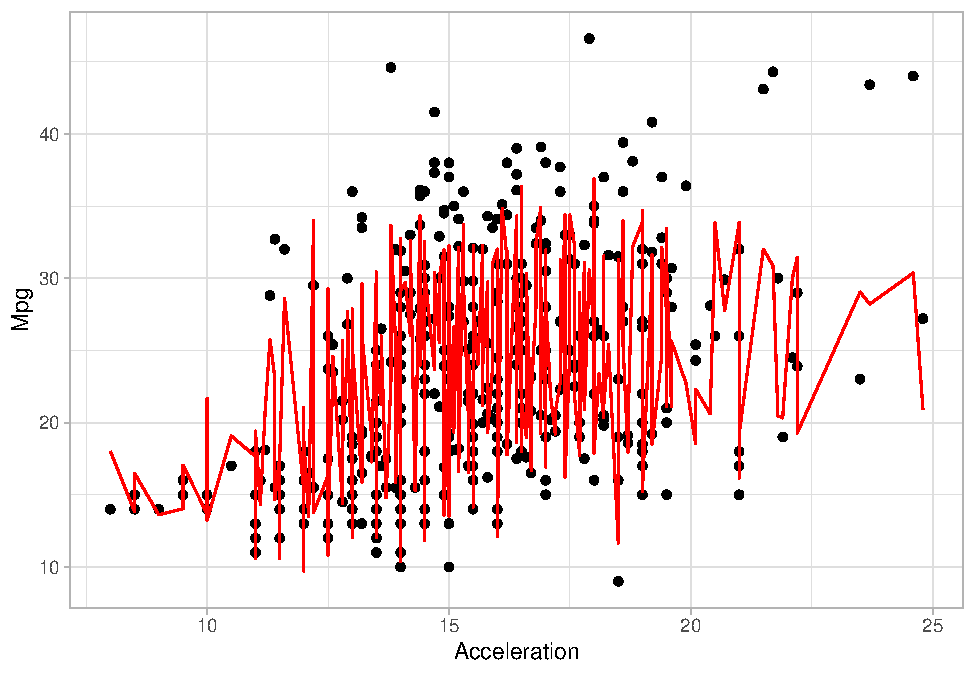
\includegraphics{Regresion_files/figure-latex/unnamed-chunk-24-2} \end{center}

\begin{Shaded}
\begin{Highlighting}[]
\NormalTok{predicted_df <-}\StringTok{ }\KeywordTok{data.frame}\NormalTok{(}\DataTypeTok{mpg_pred =} \KeywordTok{predict}\NormalTok{(fit, auto), }\DataTypeTok{hp=}\NormalTok{auto}\OperatorTok{$}\NormalTok{Displacement)}

\KeywordTok{ggplot}\NormalTok{(}\DataTypeTok{data =}\NormalTok{ auto, }\KeywordTok{aes}\NormalTok{(}\DataTypeTok{y =}\NormalTok{ Mpg, }\DataTypeTok{x =}\NormalTok{ Displacement)) }\OperatorTok{+}\StringTok{ }
\StringTok{  }\KeywordTok{geom_point}\NormalTok{() }\OperatorTok{+}
\StringTok{  }\KeywordTok{geom_line}\NormalTok{(}\DataTypeTok{color=}\StringTok{'red'}\NormalTok{, }\DataTypeTok{data =}\NormalTok{ predicted_df, }\KeywordTok{aes}\NormalTok{(}\DataTypeTok{y=}\NormalTok{mpg_pred, }\DataTypeTok{x=}\NormalTok{hp)) }\OperatorTok{+}
\StringTok{  }\KeywordTok{theme_light}\NormalTok{()}
\end{Highlighting}
\end{Shaded}

\begin{center}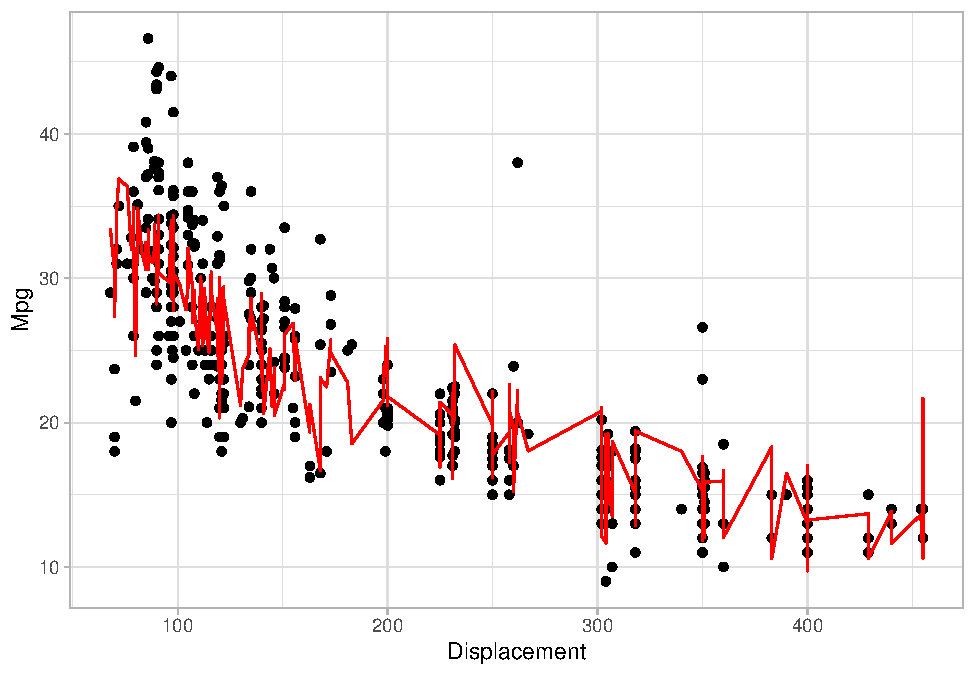
\includegraphics{Regresion_files/figure-latex/unnamed-chunk-24-3} \end{center}

Vemos un empeoramiento significativo en la calidad de R2 respecto al
modelo multivariable, pero la forma del modelo no está tan ajustada a
los datos y parece sensato mantenerlo así.

Aún así, no resulta lógico intentar predecir el Mpg de un coche
únicamente en base al peso, alguna de las otras variables deberían
ayudarnos en la predección. Por ejemplo, alguna característica del
motor, como la cilindrada o los caballos de vapor.

Para resumir, mostramos el modelo con mejor R2 tras hacer múltiples
pruebas, e intentando evitar un overfitting:

\begin{Shaded}
\begin{Highlighting}[]
\KeywordTok{lm}\NormalTok{(Mpg }\OperatorTok{~}\StringTok{ }\NormalTok{Acceleration }\OperatorTok{+}\StringTok{ }\KeywordTok{I}\NormalTok{(}\KeywordTok{log}\NormalTok{(Weight)) }\OperatorTok{+}\StringTok{ }\KeywordTok{I}\NormalTok{(}\KeywordTok{log}\NormalTok{(Displacement)), }\DataTypeTok{data=}\NormalTok{auto) }\OperatorTok\StringTok{ }
\StringTok{  }\KeywordTok{summary}\NormalTok{()}
\end{Highlighting}
\end{Shaded}

\begin{verbatim}

Call:
lm(formula = Mpg ~ Acceleration + I(log(Weight)) + I(log(Displacement)), 
    data = auto)

Residuals:
     Min       1Q   Median       3Q      Max 
-12.9074  -2.6174  -0.4104   1.9500  16.5596 

Coefficients:
                      Estimate Std. Error t value Pr(>|t|)    
(Intercept)          171.61778   12.14751  14.128  < 2e-16 ***
Acceleration           0.19717    0.08914   2.212   0.0276 *  
I(log(Weight))       -16.94003    2.27727  -7.439 6.59e-13 ***
I(log(Displacement))  -3.19963    1.26881  -2.522   0.0121 *  
---
Signif. codes:  0 '***' 0.001 '**' 0.01 '*' 0.05 '.' 0.1 ' ' 1

Residual standard error: 4.104 on 388 degrees of freedom
Multiple R-squared:  0.7256,    Adjusted R-squared:  0.7235 
F-statistic: 342.1 on 3 and 388 DF,  p-value: < 2.2e-16
\end{verbatim}

Los p-valores no son muy fuertes, pero siguen siendo aceptables, y
gráficamente el modelo se ve un poco mejor:

\begin{Shaded}
\begin{Highlighting}[]
\NormalTok{fit <-}\StringTok{ }\KeywordTok{lm}\NormalTok{(Mpg }\OperatorTok{~}\StringTok{ }\NormalTok{Acceleration }\OperatorTok{+}\StringTok{ }\KeywordTok{I}\NormalTok{(}\KeywordTok{log}\NormalTok{(Weight)) }\OperatorTok{+}\StringTok{ }\KeywordTok{I}\NormalTok{(}\KeywordTok{log}\NormalTok{(Displacement)), }\DataTypeTok{data=}\NormalTok{auto)}

\NormalTok{predicted_df <-}\StringTok{ }\KeywordTok{data.frame}\NormalTok{(}\DataTypeTok{mpg_pred =} \KeywordTok{predict}\NormalTok{(fit, auto), }\DataTypeTok{hp=}\NormalTok{auto}\OperatorTok{$}\NormalTok{Weight)}

\CommentTok{# this is the predicted line of multiple linear regression}
\KeywordTok{ggplot}\NormalTok{(}\DataTypeTok{data =}\NormalTok{ auto, }\KeywordTok{aes}\NormalTok{(}\DataTypeTok{y =}\NormalTok{ Mpg, }\DataTypeTok{x =}\NormalTok{ Weight)) }\OperatorTok{+}\StringTok{ }
\StringTok{  }\KeywordTok{geom_point}\NormalTok{() }\OperatorTok{+}
\StringTok{  }\KeywordTok{geom_line}\NormalTok{(}\DataTypeTok{color=}\StringTok{'red'}\NormalTok{, }\DataTypeTok{data =}\NormalTok{ predicted_df, }\KeywordTok{aes}\NormalTok{(}\DataTypeTok{y=}\NormalTok{mpg_pred, }\DataTypeTok{x=}\NormalTok{hp)) }\OperatorTok{+}
\StringTok{  }\KeywordTok{theme_light}\NormalTok{()}
\end{Highlighting}
\end{Shaded}

\begin{center}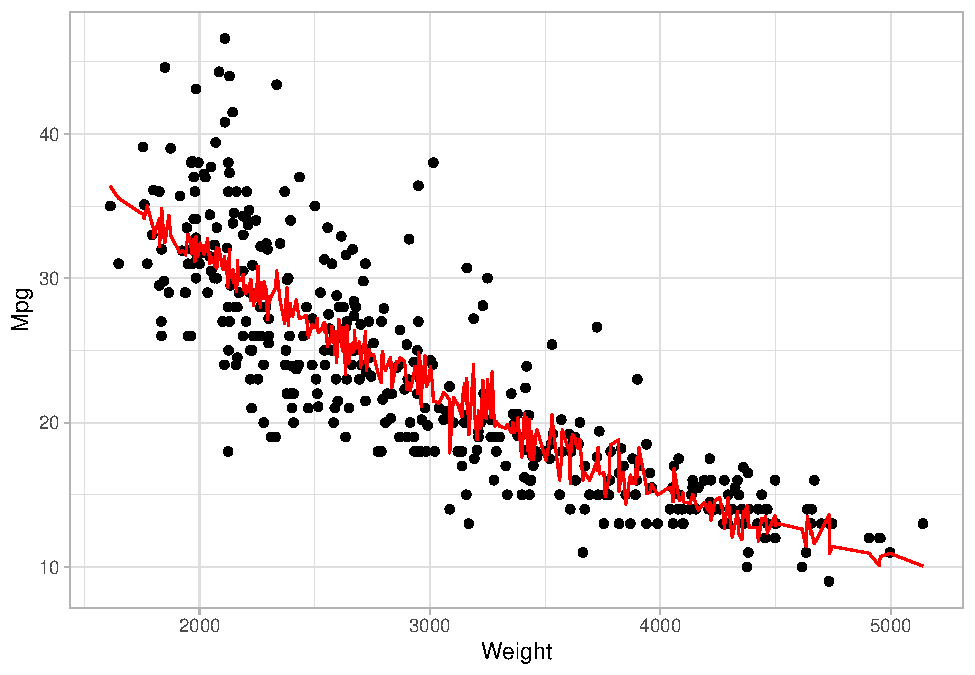
\includegraphics{Regresion_files/figure-latex/unnamed-chunk-26-1} \end{center}

\begin{Shaded}
\begin{Highlighting}[]
\NormalTok{predicted_df <-}\StringTok{ }\KeywordTok{data.frame}\NormalTok{(}\DataTypeTok{mpg_pred =} \KeywordTok{predict}\NormalTok{(fit, auto), }\DataTypeTok{hp=}\NormalTok{auto}\OperatorTok{$}\NormalTok{Acceleration)}

\KeywordTok{ggplot}\NormalTok{(}\DataTypeTok{data =}\NormalTok{ auto, }\KeywordTok{aes}\NormalTok{(}\DataTypeTok{y =}\NormalTok{ Mpg, }\DataTypeTok{x =}\NormalTok{ Acceleration)) }\OperatorTok{+}\StringTok{ }
\StringTok{  }\KeywordTok{geom_point}\NormalTok{() }\OperatorTok{+}
\StringTok{  }\KeywordTok{geom_line}\NormalTok{(}\DataTypeTok{color=}\StringTok{'red'}\NormalTok{, }\DataTypeTok{data =}\NormalTok{ predicted_df, }\KeywordTok{aes}\NormalTok{(}\DataTypeTok{y=}\NormalTok{mpg_pred, }\DataTypeTok{x=}\NormalTok{hp)) }\OperatorTok{+}
\StringTok{  }\KeywordTok{theme_light}\NormalTok{()}
\end{Highlighting}
\end{Shaded}

\begin{center}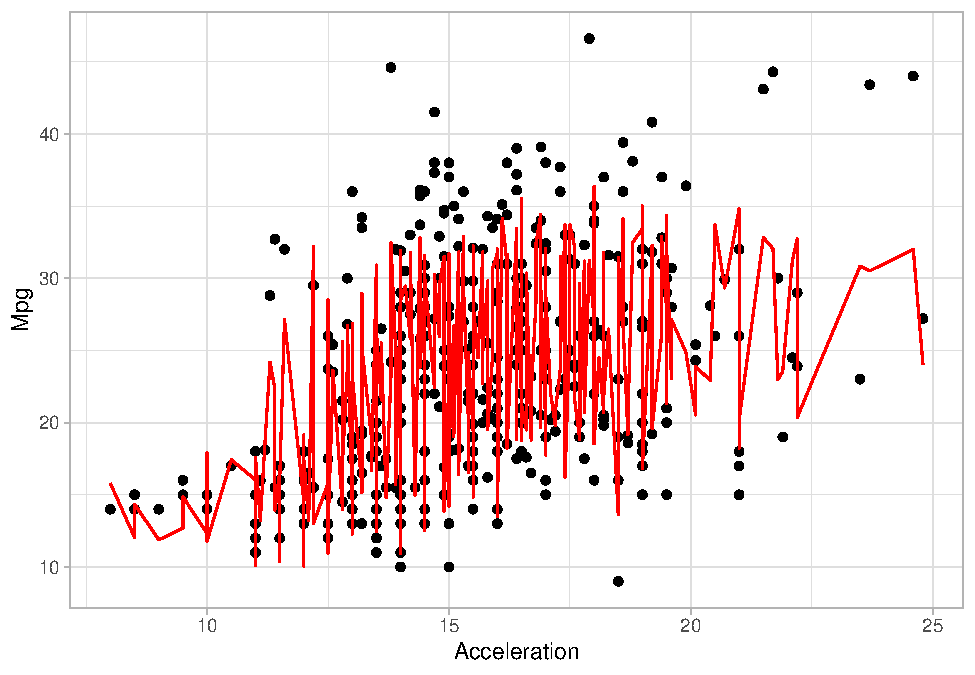
\includegraphics{Regresion_files/figure-latex/unnamed-chunk-26-2} \end{center}

\begin{Shaded}
\begin{Highlighting}[]
\NormalTok{predicted_df <-}\StringTok{ }\KeywordTok{data.frame}\NormalTok{(}\DataTypeTok{mpg_pred =} \KeywordTok{predict}\NormalTok{(fit, auto), }\DataTypeTok{hp=}\NormalTok{auto}\OperatorTok{$}\NormalTok{Displacement)}

\KeywordTok{ggplot}\NormalTok{(}\DataTypeTok{data =}\NormalTok{ auto, }\KeywordTok{aes}\NormalTok{(}\DataTypeTok{y =}\NormalTok{ Mpg, }\DataTypeTok{x =}\NormalTok{ Displacement)) }\OperatorTok{+}\StringTok{ }
\StringTok{  }\KeywordTok{geom_point}\NormalTok{() }\OperatorTok{+}
\StringTok{  }\KeywordTok{geom_line}\NormalTok{(}\DataTypeTok{color=}\StringTok{'red'}\NormalTok{, }\DataTypeTok{data =}\NormalTok{ predicted_df, }\KeywordTok{aes}\NormalTok{(}\DataTypeTok{y=}\NormalTok{mpg_pred, }\DataTypeTok{x=}\NormalTok{hp)) }\OperatorTok{+}
\StringTok{  }\KeywordTok{theme_light}\NormalTok{()}
\end{Highlighting}
\end{Shaded}

\begin{center}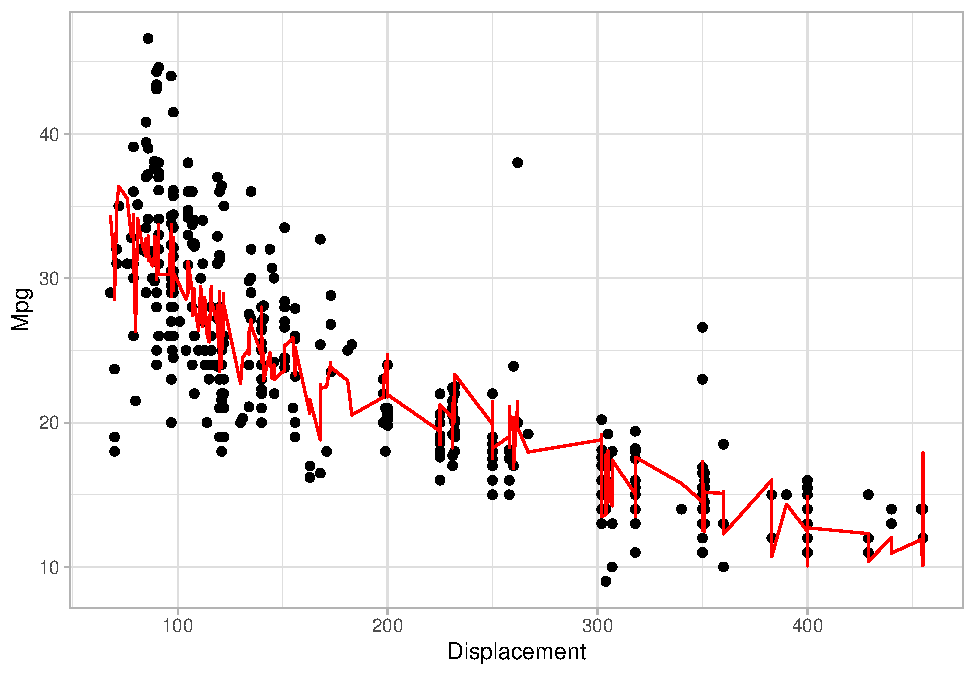
\includegraphics{Regresion_files/figure-latex/unnamed-chunk-26-3} \end{center}

Pensando en el problema, y tras el análisis hecho en el apartado de EDA,
creemos que usar Model\_year para predecir Mpg no parece buena idea. La
gráfica de la variable nos muestran mucha dispersión en los datos y,
aunque sí se ve un cierta tendencia lineal, no parece suficiente para
usarla. Claramente nos ajusta mejor los datos pero parece que nos
estamos pegando a ellos.

De cara a comprobar este razonamiento en el cross-validation, vamos a
guardar dos modelos: - Modelo con mejor R2 Mpg \textasciitilde{} Weight
+ Model\_year + I(log(Weight)

\begin{itemize}
\tightlist
\item
  Modelo intentando evitar el overfitting Mpg \textasciitilde{}
  Acceleration + I(log(Weight)) + I(log(Displacement))
\end{itemize}

\begin{center}\rule{0.5\linewidth}{0.5pt}\end{center}

\hypertarget{ajustes-con-knn}{%
\subsection{Ajustes con KNN}\label{ajustes-con-knn}}

Sabemos que la función por defecto usa la distancia de Minkowski y
escala los datos a igual rango. También usa un k de 7, y sería
recomendable probar con varios.

Vamos a probar con diferentes modelos, primero el multivariable con
todas

\begin{Shaded}
\begin{Highlighting}[]
\NormalTok{fitknn <-}\StringTok{ }\KeywordTok{kknn}\NormalTok{(Mpg}\OperatorTok{~}\NormalTok{., auto, auto)}

\NormalTok{yprime <-}\StringTok{ }\NormalTok{fitknn}\OperatorTok{$}\NormalTok{fitted.values}
\KeywordTok{sqrt}\NormalTok{(}\KeywordTok{sum}\NormalTok{((auto}\OperatorTok{$}\NormalTok{Mpg }\OperatorTok{-}\StringTok{ }\NormalTok{yprime)}\OperatorTok{^}\DecValTok{2}\NormalTok{)}\OperatorTok{/}\KeywordTok{length}\NormalTok{(yprime)) }\CommentTok{#RMSE}
\end{Highlighting}
\end{Shaded}

\begin{verbatim}
[1] 1.880835
\end{verbatim}

Y probando con varios obtenemos el menor error con este

\begin{Shaded}
\begin{Highlighting}[]
\NormalTok{fitknn <-}\StringTok{ }\KeywordTok{kknn}\NormalTok{(Mpg}\OperatorTok{~}\NormalTok{.}\OperatorTok{-}\NormalTok{Acceleration, auto, auto)}

\NormalTok{yprime <-}\StringTok{ }\NormalTok{fitknn}\OperatorTok{$}\NormalTok{fitted.values}
\KeywordTok{sqrt}\NormalTok{(}\KeywordTok{sum}\NormalTok{((auto}\OperatorTok{$}\NormalTok{Mpg }\OperatorTok{-}\StringTok{ }\NormalTok{yprime)}\OperatorTok{^}\DecValTok{2}\NormalTok{)}\OperatorTok{/}\KeywordTok{length}\NormalTok{(yprime)) }\CommentTok{#RMSE}
\end{Highlighting}
\end{Shaded}

\begin{verbatim}
[1] 1.856269
\end{verbatim}

Que visualmente nos quedaría

\begin{Shaded}
\begin{Highlighting}[]
\KeywordTok{plot}\NormalTok{(auto}\OperatorTok{$}\NormalTok{Mpg}\OperatorTok{~}\NormalTok{auto}\OperatorTok{$}\NormalTok{Weight)}
\KeywordTok{points}\NormalTok{(auto}\OperatorTok{$}\NormalTok{Weight,fitknn}\OperatorTok{$}\NormalTok{fitted.values,}\DataTypeTok{col=}\StringTok{"blue"}\NormalTok{,}\DataTypeTok{pch=}\DecValTok{20}\NormalTok{)}
\end{Highlighting}
\end{Shaded}

\begin{center}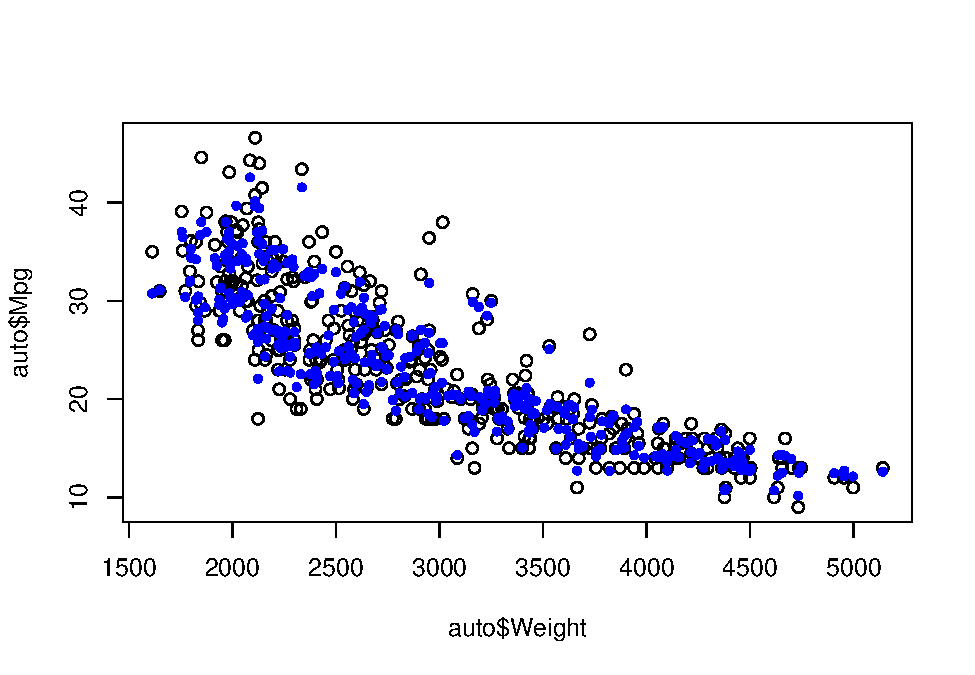
\includegraphics{Regresion_files/figure-latex/unnamed-chunk-29-1} \end{center}

\begin{Shaded}
\begin{Highlighting}[]
\KeywordTok{plot}\NormalTok{(auto}\OperatorTok{$}\NormalTok{Mpg}\OperatorTok{~}\NormalTok{auto}\OperatorTok{$}\NormalTok{Acceleration)}
\KeywordTok{points}\NormalTok{(auto}\OperatorTok{$}\NormalTok{Acceleration,fitknn}\OperatorTok{$}\NormalTok{fitted.values,}\DataTypeTok{col=}\StringTok{"blue"}\NormalTok{,}\DataTypeTok{pch=}\DecValTok{20}\NormalTok{)}
\end{Highlighting}
\end{Shaded}

\begin{center}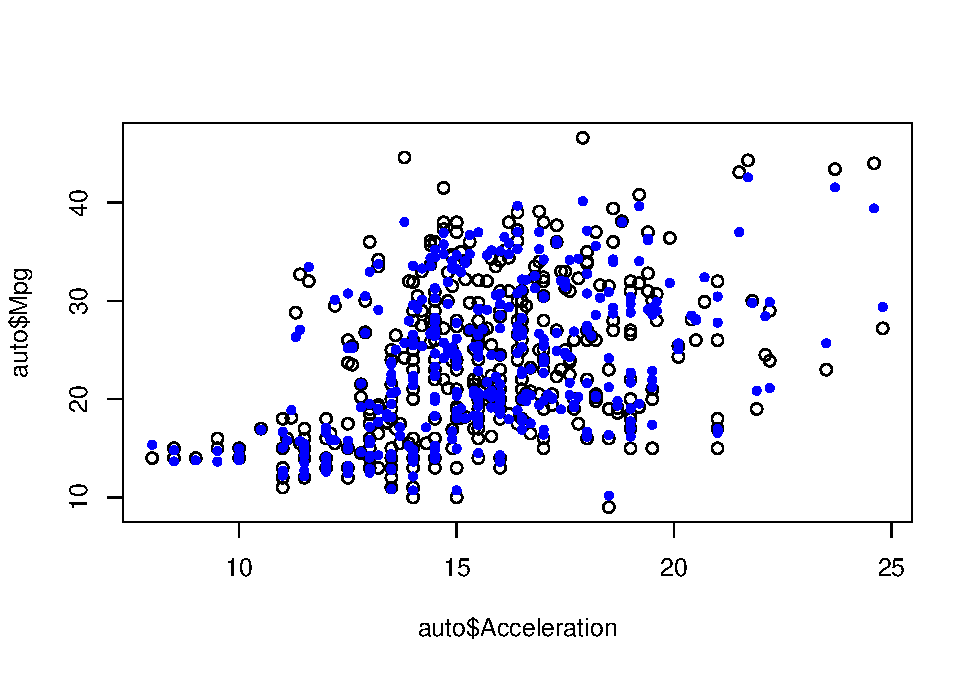
\includegraphics{Regresion_files/figure-latex/unnamed-chunk-29-2} \end{center}

Si probamos el modelo no lineal obtenido en los pasos anteriores (con
mejor R2)

\begin{Shaded}
\begin{Highlighting}[]
\NormalTok{fitknn <-}\StringTok{ }\KeywordTok{kknn}\NormalTok{(Mpg }\OperatorTok{~}\StringTok{ }\NormalTok{Weight }\OperatorTok{+}\StringTok{ }\NormalTok{Model_year }\OperatorTok{+}\StringTok{ }\KeywordTok{I}\NormalTok{(}\KeywordTok{log}\NormalTok{(Weight)), auto, auto)}

\NormalTok{yprime <-}\StringTok{ }\NormalTok{fitknn}\OperatorTok{$}\NormalTok{fitted.values}
\KeywordTok{sqrt}\NormalTok{(}\KeywordTok{sum}\NormalTok{((auto}\OperatorTok{$}\NormalTok{Mpg }\OperatorTok{-}\StringTok{ }\NormalTok{yprime)}\OperatorTok{^}\DecValTok{2}\NormalTok{)}\OperatorTok{/}\KeywordTok{length}\NormalTok{(yprime)) }\CommentTok{#RMSE}
\end{Highlighting}
\end{Shaded}

\begin{verbatim}
[1] 2.104086
\end{verbatim}

Nos da peor error.

Y si probamos el modelo no lineal en el que intemos resolver el
overfitting

\begin{Shaded}
\begin{Highlighting}[]
\NormalTok{fitknn2 <-}\StringTok{ }\KeywordTok{kknn}\NormalTok{(Mpg }\OperatorTok{~}\StringTok{ }\NormalTok{Acceleration }\OperatorTok{+}\StringTok{ }\KeywordTok{I}\NormalTok{(}\KeywordTok{log}\NormalTok{(Weight)) }\OperatorTok{+}\StringTok{ }\KeywordTok{I}\NormalTok{(}\KeywordTok{log}\NormalTok{(Displacement)), auto, auto)}

\NormalTok{yprime <-}\StringTok{ }\NormalTok{fitknn2}\OperatorTok{$}\NormalTok{fitted.values}
\KeywordTok{sqrt}\NormalTok{(}\KeywordTok{sum}\NormalTok{((auto}\OperatorTok{$}\NormalTok{Mpg }\OperatorTok{-}\StringTok{ }\NormalTok{yprime)}\OperatorTok{^}\DecValTok{2}\NormalTok{)}\OperatorTok{/}\KeywordTok{length}\NormalTok{(yprime)) }\CommentTok{#RMSE}
\end{Highlighting}
\end{Shaded}

\begin{verbatim}
[1] 2.938051
\end{verbatim}

Obtenemos aún mayor empeoramiento. Gráficamente:

\begin{Shaded}
\begin{Highlighting}[]
\KeywordTok{plot}\NormalTok{(auto}\OperatorTok{$}\NormalTok{Mpg}\OperatorTok{~}\NormalTok{auto}\OperatorTok{$}\NormalTok{Weight)}
\KeywordTok{points}\NormalTok{(auto}\OperatorTok{$}\NormalTok{Weight,fitknn}\OperatorTok{$}\NormalTok{fitted.values,}\DataTypeTok{col=}\StringTok{"red"}\NormalTok{,}\DataTypeTok{pch=}\DecValTok{20}\NormalTok{)}
\end{Highlighting}
\end{Shaded}

\begin{center}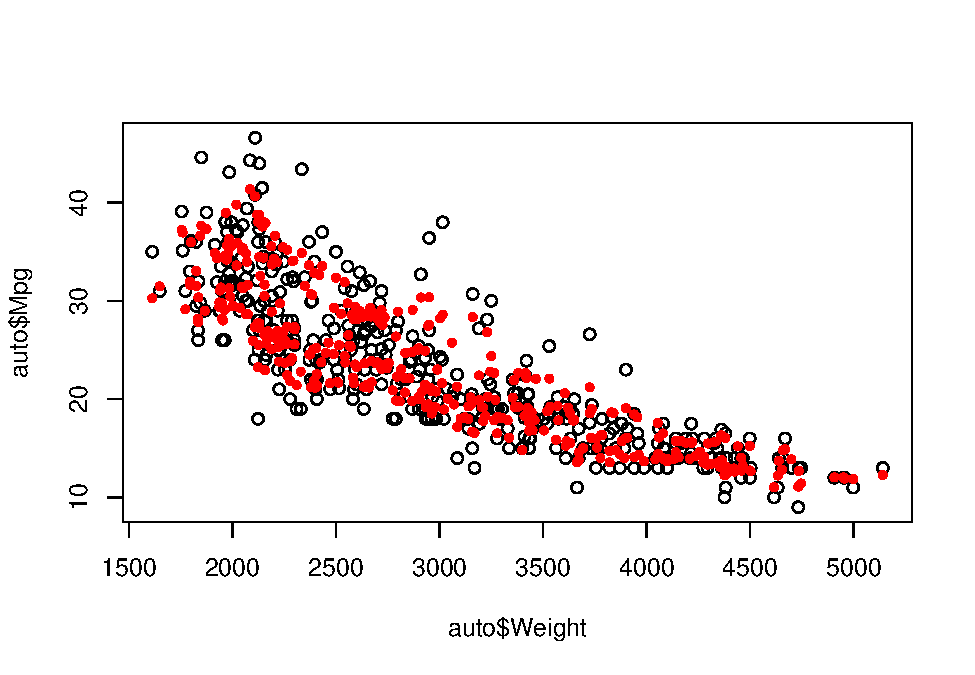
\includegraphics{Regresion_files/figure-latex/unnamed-chunk-32-1} \end{center}

\begin{Shaded}
\begin{Highlighting}[]
\KeywordTok{plot}\NormalTok{(auto}\OperatorTok{$}\NormalTok{Mpg}\OperatorTok{~}\NormalTok{auto}\OperatorTok{$}\NormalTok{Acceleration)}
\KeywordTok{points}\NormalTok{(auto}\OperatorTok{$}\NormalTok{Acceleration,fitknn2}\OperatorTok{$}\NormalTok{fitted.values,}\DataTypeTok{col=}\StringTok{"blue"}\NormalTok{,}\DataTypeTok{pch=}\DecValTok{20}\NormalTok{)}
\end{Highlighting}
\end{Shaded}

\begin{center}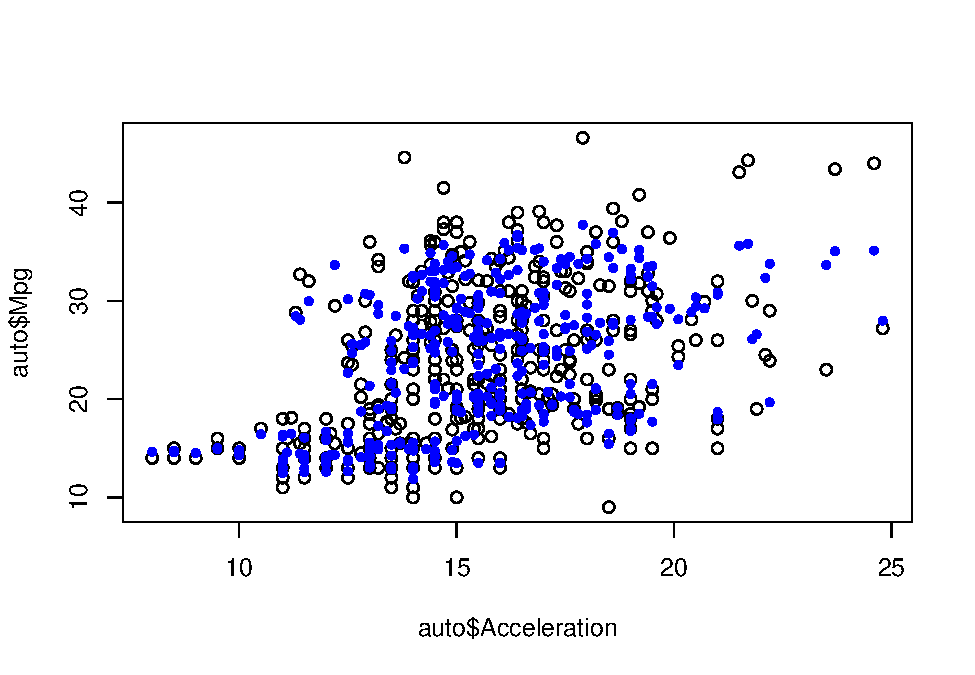
\includegraphics{Regresion_files/figure-latex/unnamed-chunk-32-2} \end{center}

El RMSE (Root Mean Square Error) o raíz del error cuadrático medio nos
permite calcular el error en nuestro conjunto de test o training
producido en las predicciones, definido por la fórmula:

El método para evitar el overfitting que usamos en el apartado anterior
probablemente no funcione con KNN por seguir una metodología totalmente
diferente. El ajuste de KNN para regresión no tiene nada que ver con los
modelos LM. Podemos aún así guardarlo para comprobarlo.

Tendríamos por tanto los siguientes modelos para KNN: Mpg
\textasciitilde{} . - Acceleration Mpg \textasciitilde{} Acceleration +
I(log(Weight)) + I(log(Displacement))

Comparandolos gráficamente, vemos que son similares

\begin{Shaded}
\begin{Highlighting}[]
\NormalTok{fitknn <-}\StringTok{ }\KeywordTok{kknn}\NormalTok{(Mpg }\OperatorTok{~}\StringTok{ }\NormalTok{. }\OperatorTok{-}\StringTok{ }\NormalTok{Acceleration, auto, auto)}
\NormalTok{fitknn2 <-}\StringTok{ }\KeywordTok{kknn}\NormalTok{(Mpg }\OperatorTok{~}\StringTok{ }\NormalTok{Acceleration }\OperatorTok{+}\StringTok{ }\KeywordTok{I}\NormalTok{(}\KeywordTok{log}\NormalTok{(Weight)) }\OperatorTok{+}\StringTok{ }\KeywordTok{I}\NormalTok{(}\KeywordTok{log}\NormalTok{(Displacement)), auto, auto)}

\KeywordTok{plot}\NormalTok{(auto}\OperatorTok{$}\NormalTok{Mpg}\OperatorTok{~}\NormalTok{auto}\OperatorTok{$}\NormalTok{Weight)}
\KeywordTok{points}\NormalTok{(auto}\OperatorTok{$}\NormalTok{Weight,fitknn}\OperatorTok{$}\NormalTok{fitted.values,}\DataTypeTok{col=}\StringTok{"red"}\NormalTok{,}\DataTypeTok{pch=}\DecValTok{20}\NormalTok{)}
\KeywordTok{points}\NormalTok{(auto}\OperatorTok{$}\NormalTok{Weight,fitknn2}\OperatorTok{$}\NormalTok{fitted.values,}\DataTypeTok{col=}\StringTok{"blue"}\NormalTok{,}\DataTypeTok{pch=}\DecValTok{20}\NormalTok{)}
\end{Highlighting}
\end{Shaded}

\begin{center}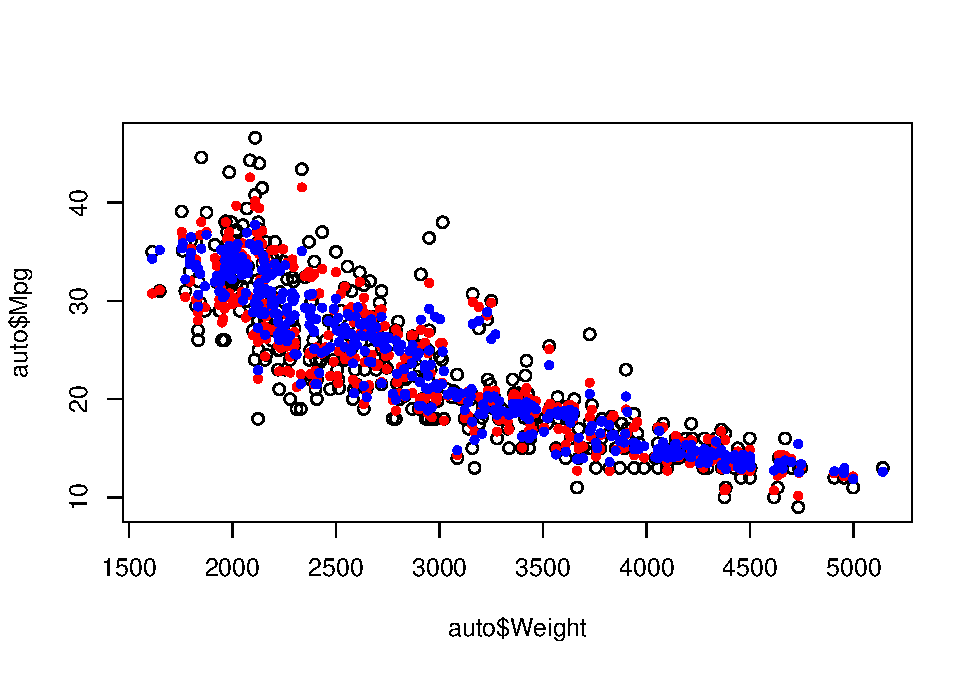
\includegraphics{Regresion_files/figure-latex/unnamed-chunk-33-1} \end{center}

\begin{Shaded}
\begin{Highlighting}[]
\KeywordTok{plot}\NormalTok{(auto}\OperatorTok{$}\NormalTok{Mpg}\OperatorTok{~}\NormalTok{auto}\OperatorTok{$}\NormalTok{Acceleration)}
\KeywordTok{points}\NormalTok{(auto}\OperatorTok{$}\NormalTok{Acceleration,fitknn}\OperatorTok{$}\NormalTok{fitted.values,}\DataTypeTok{col=}\StringTok{"red"}\NormalTok{,}\DataTypeTok{pch=}\DecValTok{20}\NormalTok{)}
\KeywordTok{points}\NormalTok{(auto}\OperatorTok{$}\NormalTok{Acceleration,fitknn2}\OperatorTok{$}\NormalTok{fitted.values,}\DataTypeTok{col=}\StringTok{"blue"}\NormalTok{,}\DataTypeTok{pch=}\DecValTok{20}\NormalTok{)}
\end{Highlighting}
\end{Shaded}

\begin{center}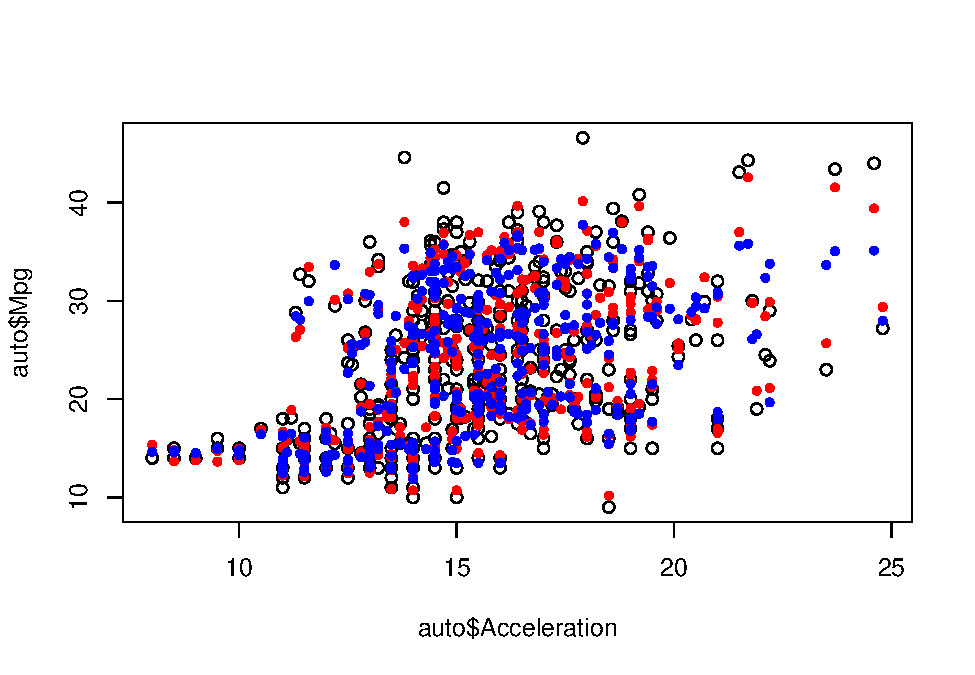
\includegraphics{Regresion_files/figure-latex/unnamed-chunk-33-2} \end{center}

Aunque el que intenta evitar el overfitting (en color azul en la
gráfica), tiene menor dispersión.

\begin{center}\rule{0.5\linewidth}{0.5pt}\end{center}

\hypertarget{comparativa-de-los-ajustes-anteriores-con-cross-validation}{%
\subsection{Comparativa de los ajustes anteriores con
cross-validation}\label{comparativa-de-los-ajustes-anteriores-con-cross-validation}}

Recordamos los modelos obtenidos: LM: Mpg \textasciitilde{} Weight +
Model\_year + I(log(Weight) Mpg \textasciitilde{} Acceleration +
I(log(Weight)) + I(log(Displacement))

KNN: Mpg \textasciitilde{} . - Acceleration Mpg \textasciitilde{}
Acceleration + I(log(Weight)) + I(log(Displacement))

c(``Displacement'', ``Horse\_power'', ``Weight'', ``Acceleration'',
``Model\_year'', ``Mpg'') X1 X2 X3 X4 X5 Y

LM: Y \textasciitilde{} X3 + X5 + I(log(X3)) Y \textasciitilde{} X4 +
I(log(X3)) + I(log(X1))

KNN: Y \textasciitilde{} . - X4 Y \textasciitilde{} X4 + I(log(X3)) +
I(log(X1))

\begin{Shaded}
\begin{Highlighting}[]
\NormalTok{nombre <-}\StringTok{ "Data/autoMPG6/autoMPG6"}
\end{Highlighting}
\end{Shaded}

Modelo de regresión con mejor R2

\begin{Shaded}
\begin{Highlighting}[]
\CommentTok{#------------- 5-fold cross-validation LM todas las variables}
\NormalTok{run_lm_fold <-}\StringTok{ }\ControlFlowTok{function}\NormalTok{(i, x, }\DataTypeTok{tt =} \StringTok{"test"}\NormalTok{) \{}
\NormalTok{    file <-}\StringTok{ }\KeywordTok{paste}\NormalTok{(x, }\StringTok{"-5-"}\NormalTok{, i, }\StringTok{"tra.dat"}\NormalTok{, }\DataTypeTok{sep=}\StringTok{""}\NormalTok{)}
\NormalTok{    x_tra <-}\StringTok{ }\KeywordTok{read.csv}\NormalTok{(file, }\DataTypeTok{comment.char=}\StringTok{"@"}\NormalTok{, }\DataTypeTok{header=}\OtherTok{FALSE}\NormalTok{)}
\NormalTok{    file <-}\StringTok{ }\KeywordTok{paste}\NormalTok{(x, }\StringTok{"-5-"}\NormalTok{, i, }\StringTok{"tst.dat"}\NormalTok{, }\DataTypeTok{sep=}\StringTok{""}\NormalTok{)}
\NormalTok{    x_tst <-}\StringTok{ }\KeywordTok{read.csv}\NormalTok{(file, }\DataTypeTok{comment.char=}\StringTok{"@"}\NormalTok{, }\DataTypeTok{header=}\OtherTok{FALSE}\NormalTok{)}
\NormalTok{    In <-}\StringTok{ }\KeywordTok{length}\NormalTok{(}\KeywordTok{names}\NormalTok{(x_tra)) }\OperatorTok{-}\StringTok{ }\DecValTok{1}
    
    \KeywordTok{names}\NormalTok{(x_tra)[}\DecValTok{1}\OperatorTok{:}\NormalTok{In] <-}\StringTok{ }\KeywordTok{paste}\NormalTok{ (}\StringTok{"X"}\NormalTok{, }\DecValTok{1}\OperatorTok{:}\NormalTok{In, }\DataTypeTok{sep=}\StringTok{""}\NormalTok{)}
    \KeywordTok{names}\NormalTok{(x_tra)[In}\OperatorTok{+}\DecValTok{1}\NormalTok{] <-}\StringTok{ "Y"}
    \KeywordTok{names}\NormalTok{(x_tst)[}\DecValTok{1}\OperatorTok{:}\NormalTok{In] <-}\StringTok{ }\KeywordTok{paste}\NormalTok{ (}\StringTok{"X"}\NormalTok{, }\DecValTok{1}\OperatorTok{:}\NormalTok{In, }\DataTypeTok{sep=}\StringTok{""}\NormalTok{)}
    \KeywordTok{names}\NormalTok{(x_tst)[In}\OperatorTok{+}\DecValTok{1}\NormalTok{] <-}\StringTok{ "Y"}
    
    \ControlFlowTok{if}\NormalTok{ (tt }\OperatorTok{==}\StringTok{ "train"}\NormalTok{) \{}
\NormalTok{        test <-}\StringTok{ }\NormalTok{x_tra}
\NormalTok{    \}}
    \ControlFlowTok{else}\NormalTok{ \{}
\NormalTok{        test <-}\StringTok{ }\NormalTok{x_tst}
\NormalTok{    \}}
    
\NormalTok{    fitMulti=}\KeywordTok{lm}\NormalTok{(Y }\OperatorTok{~}\StringTok{ }\NormalTok{X3 }\OperatorTok{+}\StringTok{ }\NormalTok{X5 }\OperatorTok{+}\StringTok{ }\KeywordTok{I}\NormalTok{(}\KeywordTok{log}\NormalTok{(X3)),x_tra)  }\CommentTok{# Poner la fórmula aquí}
    
\NormalTok{    yprime=}\KeywordTok{predict}\NormalTok{(fitMulti,test)}
    \KeywordTok{sum}\NormalTok{(}\KeywordTok{abs}\NormalTok{(test}\OperatorTok{$}\NormalTok{Y}\OperatorTok{-}\NormalTok{yprime)}\OperatorTok{^}\DecValTok{2}\NormalTok{)}\OperatorTok{/}\KeywordTok{length}\NormalTok{(yprime) }\CommentTok{## RMSE}
\NormalTok{\}}

\NormalTok{lmMSEtrain1 <-}\StringTok{ }\KeywordTok{mean}\NormalTok{(}\KeywordTok{sapply}\NormalTok{(}\DecValTok{1}\OperatorTok{:}\DecValTok{5}\NormalTok{,run_lm_fold,nombre,}\StringTok{"train"}\NormalTok{))}
\NormalTok{lmMSEtest1 <-}\StringTok{ }\KeywordTok{mean}\NormalTok{(}\KeywordTok{sapply}\NormalTok{(}\DecValTok{1}\OperatorTok{:}\DecValTok{5}\NormalTok{,run_lm_fold,nombre,}\StringTok{"test"}\NormalTok{))}
\end{Highlighting}
\end{Shaded}

Modelo de regresión evitando overfitting

\begin{Shaded}
\begin{Highlighting}[]
\CommentTok{#------------- 5-fold cross-validation LM todas las variables}
\NormalTok{run_lm_fold <-}\StringTok{ }\ControlFlowTok{function}\NormalTok{(i, x, }\DataTypeTok{tt =} \StringTok{"test"}\NormalTok{) \{}
\NormalTok{    file <-}\StringTok{ }\KeywordTok{paste}\NormalTok{(x, }\StringTok{"-5-"}\NormalTok{, i, }\StringTok{"tra.dat"}\NormalTok{, }\DataTypeTok{sep=}\StringTok{""}\NormalTok{)}
\NormalTok{    x_tra <-}\StringTok{ }\KeywordTok{read.csv}\NormalTok{(file, }\DataTypeTok{comment.char=}\StringTok{"@"}\NormalTok{, }\DataTypeTok{header=}\OtherTok{FALSE}\NormalTok{)}
\NormalTok{    file <-}\StringTok{ }\KeywordTok{paste}\NormalTok{(x, }\StringTok{"-5-"}\NormalTok{, i, }\StringTok{"tst.dat"}\NormalTok{, }\DataTypeTok{sep=}\StringTok{""}\NormalTok{)}
\NormalTok{    x_tst <-}\StringTok{ }\KeywordTok{read.csv}\NormalTok{(file, }\DataTypeTok{comment.char=}\StringTok{"@"}\NormalTok{, }\DataTypeTok{header=}\OtherTok{FALSE}\NormalTok{)}
\NormalTok{    In <-}\StringTok{ }\KeywordTok{length}\NormalTok{(}\KeywordTok{names}\NormalTok{(x_tra)) }\OperatorTok{-}\StringTok{ }\DecValTok{1}
    
    \KeywordTok{names}\NormalTok{(x_tra)[}\DecValTok{1}\OperatorTok{:}\NormalTok{In] <-}\StringTok{ }\KeywordTok{paste}\NormalTok{ (}\StringTok{"X"}\NormalTok{, }\DecValTok{1}\OperatorTok{:}\NormalTok{In, }\DataTypeTok{sep=}\StringTok{""}\NormalTok{)}
    \KeywordTok{names}\NormalTok{(x_tra)[In}\OperatorTok{+}\DecValTok{1}\NormalTok{] <-}\StringTok{ "Y"}
    \KeywordTok{names}\NormalTok{(x_tst)[}\DecValTok{1}\OperatorTok{:}\NormalTok{In] <-}\StringTok{ }\KeywordTok{paste}\NormalTok{ (}\StringTok{"X"}\NormalTok{, }\DecValTok{1}\OperatorTok{:}\NormalTok{In, }\DataTypeTok{sep=}\StringTok{""}\NormalTok{)}
    \KeywordTok{names}\NormalTok{(x_tst)[In}\OperatorTok{+}\DecValTok{1}\NormalTok{] <-}\StringTok{ "Y"}
    
    \ControlFlowTok{if}\NormalTok{ (tt }\OperatorTok{==}\StringTok{ "train"}\NormalTok{) \{}
\NormalTok{        test <-}\StringTok{ }\NormalTok{x_tra}
\NormalTok{    \}}
    \ControlFlowTok{else}\NormalTok{ \{}
\NormalTok{        test <-}\StringTok{ }\NormalTok{x_tst}
\NormalTok{    \}}
    
\NormalTok{    fitMulti=}\KeywordTok{lm}\NormalTok{(Y }\OperatorTok{~}\StringTok{ }\NormalTok{X4 }\OperatorTok{+}\StringTok{ }\KeywordTok{I}\NormalTok{(}\KeywordTok{log}\NormalTok{(X3)) }\OperatorTok{+}\StringTok{ }\KeywordTok{I}\NormalTok{(}\KeywordTok{log}\NormalTok{(X1)),x_tra)  }\CommentTok{# Poner la fórmula aquí}
    
\NormalTok{    yprime=}\KeywordTok{predict}\NormalTok{(fitMulti,test)}
    \KeywordTok{sum}\NormalTok{(}\KeywordTok{abs}\NormalTok{(test}\OperatorTok{$}\NormalTok{Y}\OperatorTok{-}\NormalTok{yprime)}\OperatorTok{^}\DecValTok{2}\NormalTok{)}\OperatorTok{/}\KeywordTok{length}\NormalTok{(yprime) }\CommentTok{## RMSE}
\NormalTok{\}}

\NormalTok{lmMSEtrain2 <-}\StringTok{ }\KeywordTok{mean}\NormalTok{(}\KeywordTok{sapply}\NormalTok{(}\DecValTok{1}\OperatorTok{:}\DecValTok{5}\NormalTok{,run_lm_fold,nombre,}\StringTok{"train"}\NormalTok{))}
\NormalTok{lmMSEtest2 <-}\StringTok{ }\KeywordTok{mean}\NormalTok{(}\KeywordTok{sapply}\NormalTok{(}\DecValTok{1}\OperatorTok{:}\DecValTok{5}\NormalTok{,run_lm_fold,nombre,}\StringTok{"test"}\NormalTok{))}
\end{Highlighting}
\end{Shaded}

Modelo KNN con menor RSME

\begin{Shaded}
\begin{Highlighting}[]
\CommentTok{#------------- 5-fold cross-validation KNN todas las variables}
\NormalTok{run_knn_fold <-}\StringTok{ }\ControlFlowTok{function}\NormalTok{(i, x, }\DataTypeTok{tt =} \StringTok{"test"}\NormalTok{) \{}
\NormalTok{    file <-}\StringTok{ }\KeywordTok{paste}\NormalTok{(x, }\StringTok{"-5-"}\NormalTok{, i, }\StringTok{"tra.dat"}\NormalTok{, }\DataTypeTok{sep=}\StringTok{""}\NormalTok{)}
\NormalTok{    x_tra <-}\StringTok{ }\KeywordTok{read.csv}\NormalTok{(file, }\DataTypeTok{comment.char=}\StringTok{"@"}\NormalTok{, }\DataTypeTok{header=}\OtherTok{FALSE}\NormalTok{)}
\NormalTok{    file <-}\StringTok{ }\KeywordTok{paste}\NormalTok{(x, }\StringTok{"-5-"}\NormalTok{, i, }\StringTok{"tst.dat"}\NormalTok{, }\DataTypeTok{sep=}\StringTok{""}\NormalTok{)}
\NormalTok{    x_tst <-}\StringTok{ }\KeywordTok{read.csv}\NormalTok{(file, }\DataTypeTok{comment.char=}\StringTok{"@"}\NormalTok{, }\DataTypeTok{header=}\OtherTok{FALSE}\NormalTok{)}
\NormalTok{    In <-}\StringTok{ }\KeywordTok{length}\NormalTok{(}\KeywordTok{names}\NormalTok{(x_tra)) }\OperatorTok{-}\StringTok{ }\DecValTok{1}
    
    \KeywordTok{names}\NormalTok{(x_tra)[}\DecValTok{1}\OperatorTok{:}\NormalTok{In] <-}\StringTok{ }\KeywordTok{paste}\NormalTok{ (}\StringTok{"X"}\NormalTok{, }\DecValTok{1}\OperatorTok{:}\NormalTok{In, }\DataTypeTok{sep=}\StringTok{""}\NormalTok{)}
    \KeywordTok{names}\NormalTok{(x_tra)[In}\OperatorTok{+}\DecValTok{1}\NormalTok{] <-}\StringTok{ "Y"}
    \KeywordTok{names}\NormalTok{(x_tst)[}\DecValTok{1}\OperatorTok{:}\NormalTok{In] <-}\StringTok{ }\KeywordTok{paste}\NormalTok{ (}\StringTok{"X"}\NormalTok{, }\DecValTok{1}\OperatorTok{:}\NormalTok{In, }\DataTypeTok{sep=}\StringTok{""}\NormalTok{)}
    \KeywordTok{names}\NormalTok{(x_tst)[In}\OperatorTok{+}\DecValTok{1}\NormalTok{] <-}\StringTok{ "Y"}
    
    \ControlFlowTok{if}\NormalTok{ (tt }\OperatorTok{==}\StringTok{ "train"}\NormalTok{) \{}
\NormalTok{        test <-}\StringTok{ }\NormalTok{x_tra}
\NormalTok{    \}}
    \ControlFlowTok{else}\NormalTok{ \{}
\NormalTok{        test <-}\StringTok{ }\NormalTok{x_tst}
\NormalTok{    \}}
    
\NormalTok{    fitMulti=}\KeywordTok{kknn}\NormalTok{(Y }\OperatorTok{~}\StringTok{ }\NormalTok{. }\OperatorTok{-}\StringTok{ }\NormalTok{X4,x_tra,test)  }\CommentTok{# Poner la fórmula aquí}
    
\NormalTok{    yprime=fitMulti}\OperatorTok{$}\NormalTok{fitted.values}
    \KeywordTok{sum}\NormalTok{(}\KeywordTok{abs}\NormalTok{(test}\OperatorTok{$}\NormalTok{Y}\OperatorTok{-}\NormalTok{yprime)}\OperatorTok{^}\DecValTok{2}\NormalTok{)}\OperatorTok{/}\KeywordTok{length}\NormalTok{(yprime) }\CommentTok{##RMSE}
\NormalTok{\}}

\NormalTok{knnMSEtrain1 <-}\StringTok{ }\KeywordTok{mean}\NormalTok{(}\KeywordTok{sapply}\NormalTok{(}\DecValTok{1}\OperatorTok{:}\DecValTok{5}\NormalTok{,run_knn_fold,nombre,}\StringTok{"train"}\NormalTok{))}
\NormalTok{knnMSEtest1 <-}\StringTok{ }\KeywordTok{mean}\NormalTok{(}\KeywordTok{sapply}\NormalTok{(}\DecValTok{1}\OperatorTok{:}\DecValTok{5}\NormalTok{,run_knn_fold,nombre,}\StringTok{"test"}\NormalTok{))}
\end{Highlighting}
\end{Shaded}

Modelo KNN evitando overfitting

\begin{Shaded}
\begin{Highlighting}[]
\CommentTok{#------------- 5-fold cross-validation KNN todas las variables}
\NormalTok{run_knn_fold <-}\StringTok{ }\ControlFlowTok{function}\NormalTok{(i, x, }\DataTypeTok{tt =} \StringTok{"test"}\NormalTok{) \{}
\NormalTok{    file <-}\StringTok{ }\KeywordTok{paste}\NormalTok{(x, }\StringTok{"-5-"}\NormalTok{, i, }\StringTok{"tra.dat"}\NormalTok{, }\DataTypeTok{sep=}\StringTok{""}\NormalTok{)}
\NormalTok{    x_tra <-}\StringTok{ }\KeywordTok{read.csv}\NormalTok{(file, }\DataTypeTok{comment.char=}\StringTok{"@"}\NormalTok{, }\DataTypeTok{header=}\OtherTok{FALSE}\NormalTok{)}
\NormalTok{    file <-}\StringTok{ }\KeywordTok{paste}\NormalTok{(x, }\StringTok{"-5-"}\NormalTok{, i, }\StringTok{"tst.dat"}\NormalTok{, }\DataTypeTok{sep=}\StringTok{""}\NormalTok{)}
\NormalTok{    x_tst <-}\StringTok{ }\KeywordTok{read.csv}\NormalTok{(file, }\DataTypeTok{comment.char=}\StringTok{"@"}\NormalTok{, }\DataTypeTok{header=}\OtherTok{FALSE}\NormalTok{)}
\NormalTok{    In <-}\StringTok{ }\KeywordTok{length}\NormalTok{(}\KeywordTok{names}\NormalTok{(x_tra)) }\OperatorTok{-}\StringTok{ }\DecValTok{1}
    
    \KeywordTok{names}\NormalTok{(x_tra)[}\DecValTok{1}\OperatorTok{:}\NormalTok{In] <-}\StringTok{ }\KeywordTok{paste}\NormalTok{ (}\StringTok{"X"}\NormalTok{, }\DecValTok{1}\OperatorTok{:}\NormalTok{In, }\DataTypeTok{sep=}\StringTok{""}\NormalTok{)}
    \KeywordTok{names}\NormalTok{(x_tra)[In}\OperatorTok{+}\DecValTok{1}\NormalTok{] <-}\StringTok{ "Y"}
    \KeywordTok{names}\NormalTok{(x_tst)[}\DecValTok{1}\OperatorTok{:}\NormalTok{In] <-}\StringTok{ }\KeywordTok{paste}\NormalTok{ (}\StringTok{"X"}\NormalTok{, }\DecValTok{1}\OperatorTok{:}\NormalTok{In, }\DataTypeTok{sep=}\StringTok{""}\NormalTok{)}
    \KeywordTok{names}\NormalTok{(x_tst)[In}\OperatorTok{+}\DecValTok{1}\NormalTok{] <-}\StringTok{ "Y"}
    
    \ControlFlowTok{if}\NormalTok{ (tt }\OperatorTok{==}\StringTok{ "train"}\NormalTok{) \{}
\NormalTok{        test <-}\StringTok{ }\NormalTok{x_tra}
\NormalTok{    \}}
    \ControlFlowTok{else}\NormalTok{ \{}
\NormalTok{        test <-}\StringTok{ }\NormalTok{x_tst}
\NormalTok{    \}}
    
\NormalTok{    fitMulti=}\KeywordTok{kknn}\NormalTok{(Y }\OperatorTok{~}\StringTok{ }\NormalTok{X4 }\OperatorTok{+}\StringTok{ }\KeywordTok{I}\NormalTok{(}\KeywordTok{log}\NormalTok{(X3)) }\OperatorTok{+}\StringTok{ }\KeywordTok{I}\NormalTok{(}\KeywordTok{log}\NormalTok{(X1)),x_tra,test)  }\CommentTok{# Poner la fórmula aquí}
    
\NormalTok{    yprime=fitMulti}\OperatorTok{$}\NormalTok{fitted.values}
    \KeywordTok{sum}\NormalTok{(}\KeywordTok{abs}\NormalTok{(test}\OperatorTok{$}\NormalTok{Y}\OperatorTok{-}\NormalTok{yprime)}\OperatorTok{^}\DecValTok{2}\NormalTok{)}\OperatorTok{/}\KeywordTok{length}\NormalTok{(yprime) }\CommentTok{##RMSE}
\NormalTok{\}}

\NormalTok{knnMSEtrain2 <-}\StringTok{ }\KeywordTok{mean}\NormalTok{(}\KeywordTok{sapply}\NormalTok{(}\DecValTok{1}\OperatorTok{:}\DecValTok{5}\NormalTok{,run_knn_fold,nombre,}\StringTok{"train"}\NormalTok{))}
\NormalTok{knnMSEtest2 <-}\StringTok{ }\KeywordTok{mean}\NormalTok{(}\KeywordTok{sapply}\NormalTok{(}\DecValTok{1}\OperatorTok{:}\DecValTok{5}\NormalTok{,run_knn_fold,nombre,}\StringTok{"test"}\NormalTok{))}
\end{Highlighting}
\end{Shaded}

Resultados obtenidos

\begin{Shaded}
\begin{Highlighting}[]
\KeywordTok{cat}\NormalTok{(}\StringTok{"Regresión 1: "}\NormalTok{)}
\NormalTok{lmMSEtest1}
\KeywordTok{cat}\NormalTok{(}\StringTok{"Regresión 2: "}\NormalTok{)}
\NormalTok{lmMSEtest2}
\KeywordTok{cat}\NormalTok{(}\StringTok{"KNN 1: "}\NormalTok{)}
\NormalTok{knnMSEtest1}
\KeywordTok{cat}\NormalTok{(}\StringTok{"KNN 2: "}\NormalTok{)}
\NormalTok{knnMSEtest2}
\end{Highlighting}
\end{Shaded}

\begin{verbatim}
Regresión 1: [1] 9.333066
Regresión 2: [1] 17.10519
KNN 1: [1] 7.291517
KNN 2: [1] 18.43846
\end{verbatim}

Con el proceso de cross-validation dividimos el dataset en N
subconjuntos (folds) y repetimos el entrenamiento N veces. Cada
entrenamiento se aplica reservando uno de los subconjuntos como test y
entrenando con el resto. Al final, el error obtenido para el modelo es
la media de los errores en cada fold. La elección del número de folds es
importante y si el problema lo permite (en términos de gasto
computacional), se debería probar con varios. En este caso hemos
utilizado 5 folds.

Con esto conseguimos no desperdiciar el conocimiento del conjunto de
test y no guiarnos por una única evaluación del modelo.

Como resultados, nos muestra que los modelos con los que obtuvimos
mejores resultados de R2 y RSME en sus apartados han acabado con mejor
RSME tras el cross-validation. También apreciamos que con KNN
conseguimos ligeramente mejores resultados.

Por completitud, mostramos también los resultados en training

\begin{Shaded}
\begin{Highlighting}[]
\KeywordTok{cat}\NormalTok{(}\StringTok{"Regresión 1: "}\NormalTok{)}
\NormalTok{lmMSEtrain1}
\KeywordTok{cat}\NormalTok{(}\StringTok{"Regresión 2: "}\NormalTok{)}
\NormalTok{lmMSEtrain2}
\KeywordTok{cat}\NormalTok{(}\StringTok{"KNN 1: "}\NormalTok{)}
\NormalTok{knnMSEtrain1}
\KeywordTok{cat}\NormalTok{(}\StringTok{"KNN 2: "}\NormalTok{)}
\NormalTok{knnMSEtrain2}
\end{Highlighting}
\end{Shaded}

\begin{verbatim}
Regresión 1: [1] 9.159891
Regresión 2: [1] 16.62285
KNN 1: [1] 3.659828
KNN 2: [1] 8.642349
\end{verbatim}

Que nos muestran que ninguno de los modelos LM estaban haciendo
overfitting, pero en cambio en KNN si existe una diferencia
significativa entre training y test.

\begin{center}\rule{0.5\linewidth}{0.5pt}\end{center}

\hypertarget{comparativa-de-tests}{%
\subsection{Comparativa de tests}\label{comparativa-de-tests}}

Para comparar los algoritmos vamos a aplicar test estadísticos en base a
los resultados obtenidos en múltiples datasets. Para asegurar la
igualdad de condiciones los algoritmos hacen uso de parámetros genéricos
y utilizan las mismas particiones de cross-validation.

Estas son las tablas de resultados que tenemos:

\begin{Shaded}
\begin{Highlighting}[]
\CommentTok{# Leemos la tabla con los errores medios de test}
\NormalTok{resultados <-}\StringTok{ }\KeywordTok{read.csv}\NormalTok{(}\StringTok{"Data/regr_test_alumnos.csv"}\NormalTok{)}
\NormalTok{tablatst <-}\StringTok{ }\KeywordTok{cbind}\NormalTok{(resultados[,}\DecValTok{2}\OperatorTok{:}\KeywordTok{dim}\NormalTok{(resultados)[}\DecValTok{2}\NormalTok{]])}
\KeywordTok{colnames}\NormalTok{(tablatst) <-}\StringTok{ }\KeywordTok{names}\NormalTok{(resultados)[}\DecValTok{2}\OperatorTok{:}\KeywordTok{dim}\NormalTok{(resultados)[}\DecValTok{2}\NormalTok{]]}
\KeywordTok{rownames}\NormalTok{(tablatst) <-}\StringTok{ }\NormalTok{resultados[,}\DecValTok{1}\NormalTok{]}

\CommentTok{# Leemos la tabla con los errores medios de entrenamiento}
\NormalTok{resultados <-}\StringTok{ }\KeywordTok{read.csv}\NormalTok{(}\StringTok{"Data/regr_train_alumnos.csv"}\NormalTok{)}
\NormalTok{tablatra <-}\StringTok{ }\KeywordTok{cbind}\NormalTok{(resultados[,}\DecValTok{2}\OperatorTok{:}\KeywordTok{dim}\NormalTok{(resultados)[}\DecValTok{2}\NormalTok{]])}
\KeywordTok{colnames}\NormalTok{(tablatra) <-}\StringTok{ }\KeywordTok{names}\NormalTok{(resultados)[}\DecValTok{2}\OperatorTok{:}\KeywordTok{dim}\NormalTok{(resultados)[}\DecValTok{2}\NormalTok{]]}
\KeywordTok{rownames}\NormalTok{(tablatra) <-}\StringTok{ }\NormalTok{resultados[,}\DecValTok{1}\NormalTok{]}

\CommentTok{# TABLA NORMALIZADA - lm (other) vs knn (ref) para WILCOXON}
\CommentTok{# + 0.1 porque wilcox R falla para valores == 0 en la tabla}

\NormalTok{difs <-}\StringTok{ }\NormalTok{(tablatst[,}\DecValTok{1}\NormalTok{] }\OperatorTok{-}\StringTok{ }\NormalTok{tablatst[,}\DecValTok{2}\NormalTok{]) }\OperatorTok{/}\StringTok{ }\NormalTok{tablatst[,}\DecValTok{1}\NormalTok{]}
\NormalTok{wilc_}\DecValTok{1}\NormalTok{_}\DecValTok{2}\NormalTok{ <-}\StringTok{ }\KeywordTok{cbind}\NormalTok{(}\KeywordTok{ifelse}\NormalTok{ (difs}\OperatorTok{<}\DecValTok{0}\NormalTok{, }\KeywordTok{abs}\NormalTok{(difs)}\OperatorTok{+}\FloatTok{0.1}\NormalTok{, }\DecValTok{0}\FloatTok{+0.1}\NormalTok{), }\KeywordTok{ifelse}\NormalTok{ (difs}\OperatorTok{>}\DecValTok{0}\NormalTok{,    }\KeywordTok{abs}\NormalTok{(difs)}\OperatorTok{+}\FloatTok{0.1}\NormalTok{, }\DecValTok{0}\FloatTok{+0.1}\NormalTok{))}
\KeywordTok{colnames}\NormalTok{(wilc_}\DecValTok{1}\NormalTok{_}\DecValTok{2}\NormalTok{) <-}\StringTok{ }\KeywordTok{c}\NormalTok{(}\KeywordTok{colnames}\NormalTok{(tablatst)[}\DecValTok{1}\NormalTok{], }\KeywordTok{colnames}\NormalTok{(tablatst)[}\DecValTok{2}\NormalTok{])}
\KeywordTok{head}\NormalTok{(wilc_}\DecValTok{1}\NormalTok{_}\DecValTok{2} \OperatorTok\StringTok{ }\KeywordTok{as.data.frame}\NormalTok{())}
\end{Highlighting}
\end{Shaded}

\begin{longtable}[]{@{}rr@{}}
\toprule
out\_test\_lm & out\_test\_kknn\tabularnewline
\midrule
\endhead
0.1909091 & 0.1000000\tabularnewline
0.1000000 & 1.0294118\tabularnewline
0.1000000 & 0.4339071\tabularnewline
0.1000000 & 0.3885965\tabularnewline
0.1548506 & 0.1000000\tabularnewline
0.1000000 & 0.3061057\tabularnewline
\bottomrule
\end{longtable}

Aplicamos el test de Wilconxon a LM y KNN

\begin{Shaded}
\begin{Highlighting}[]
\CommentTok{# Aplicación del test de WILCOXON}
\NormalTok{LMvsKNNtst <-}\StringTok{ }\KeywordTok{wilcox.test}\NormalTok{(wilc_}\DecValTok{1}\NormalTok{_}\DecValTok{2}\NormalTok{[,}\DecValTok{1}\NormalTok{], wilc_}\DecValTok{1}\NormalTok{_}\DecValTok{2}\NormalTok{[,}\DecValTok{2}\NormalTok{], }\DataTypeTok{alternative =} \StringTok{"two.sided"}\NormalTok{, }\DataTypeTok{paired=}\OtherTok{TRUE}\NormalTok{)}
\NormalTok{Rmas <-}\StringTok{ }\NormalTok{LMvsKNNtst}\OperatorTok{$}\NormalTok{statistic}

\NormalTok{pvalue <-}\StringTok{ }\NormalTok{LMvsKNNtst}\OperatorTok{$}\NormalTok{p.value}

\NormalTok{LMvsKNNtst <-}\StringTok{ }\KeywordTok{wilcox.test}\NormalTok{(wilc_}\DecValTok{1}\NormalTok{_}\DecValTok{2}\NormalTok{[,}\DecValTok{2}\NormalTok{], wilc_}\DecValTok{1}\NormalTok{_}\DecValTok{2}\NormalTok{[,}\DecValTok{1}\NormalTok{], }\DataTypeTok{alternative =} \StringTok{"two.sided"}\NormalTok{, }\DataTypeTok{paired=}\OtherTok{TRUE}\NormalTok{)}
\NormalTok{Rmenos <-}\StringTok{ }\NormalTok{LMvsKNNtst}\OperatorTok{$}\NormalTok{statistic}

\NormalTok{Rmas}
\NormalTok{Rmenos}
\KeywordTok{cat}\NormalTok{(}\StringTok{"p-value: "}\NormalTok{)}
\NormalTok{pvalue}
\end{Highlighting}
\end{Shaded}

\begin{verbatim}
 V 
78 
 V 
93 
p-value: [1] 0.7660294
\end{verbatim}

Obtenemos un ranking de 78 para LM y 93 para KNN, con un p-valor de 0.77
(o nivel de confianza del 33\%).

Esto nos dice que gana KNN pero puesto que el p-value no es lo
suficientemente grande no podemos afirmar con un nivel alto de
significación que las diferencias entre los tests sean notorias.

Ahora aplicamos en test de Friedman a los dos algoritmos anterios junto
al algoritmo M5:

\begin{Shaded}
\begin{Highlighting}[]
\CommentTok{# Aplicación del test de Friedman}
\NormalTok{test_friedman <-}\StringTok{ }\KeywordTok{friedman.test}\NormalTok{(}\KeywordTok{as.matrix}\NormalTok{(tablatst))}
\NormalTok{test_friedman}
\end{Highlighting}
\end{Shaded}

\begin{verbatim}

    Friedman rank sum test

data:  as.matrix(tablatst)
Friedman chi-squared = 8.4444, df = 2, p-value = 0.01467
\end{verbatim}

El p-value es \textless0.05 por lo que podemos concluir que al menos hay
un par de algoritmos de calidad diferente.

Vemos cuáles de ellos lo son haciendo el test post-hoc de HOLM

\begin{Shaded}
\begin{Highlighting}[]
\CommentTok{# Aplicación del test post-hoc de HOLM}
\NormalTok{tam <-}\StringTok{ }\KeywordTok{dim}\NormalTok{(tablatst)}
\NormalTok{groups <-}\StringTok{ }\KeywordTok{rep}\NormalTok{(}\DecValTok{1}\OperatorTok{:}\NormalTok{tam[}\DecValTok{2}\NormalTok{], }\DataTypeTok{each=}\NormalTok{tam[}\DecValTok{1}\NormalTok{])}
\KeywordTok{pairwise.wilcox.test}\NormalTok{(}\KeywordTok{as.matrix}\NormalTok{(tablatst), groups, }\DataTypeTok{p.adjust =} \StringTok{"holm"}\NormalTok{, }\DataTypeTok{paired =} \OtherTok{TRUE}\NormalTok{)}
\end{Highlighting}
\end{Shaded}

\begin{verbatim}

    Pairwise comparisons using Wilcoxon signed rank exact test 

data:  as.matrix(tablatst) and groups 

  1     2    
2 0.580 -    
3 0.081 0.108

P value adjustment method: holm 
\end{verbatim}

Con el test post-hoc de HOLM podemos asegurar que 3-1 (M5 vs LM) son
diferentes. También podemos afirmar M5 respecto de KNN pero con un nivel
de confianza menor.

De KNN y LM no podemos afirmar nada puesto que el p-valor es
extremadamente grande.

\end{document}
